\documentclass[reprint,amsmath,amssymb,aps,pre]{revtex4-1}
% Latex
\usepackage[english]{babel}
\usepackage[utf8]{inputenc}
\usepackage[T1]{fontenc}
% Xelatex
%\usepackage{polyglossia}
%\usepackage{fontspec}
%\setdefaultlanguage{english}
%\setmainfont{DejaVu Sans}
%\setsansfont{DejaVu Sans}
%\setmonofont{DejaVu Sans Mono}
\usepackage{bm}
\usepackage{cleveref}
\usepackage{xcolor}
\usepackage{algpseudocode}
\usepackage{graphicx}
\usepackage{subcaption}

\definecolor{light-gray}{gray}{0.95}
\newcommand{\code}[1]{\colorbox{light-gray}{\texttt{#1}}}
% When cleveref fails to do its job
\newcommand{\apref}[1]{Appendix \ref{#1}}

\begin{document}
%*Corresponding author: Kirill M. Gerke, Tel.: +79661877715, E-mail: kg@ifz.ru,
%Address: Schmidt Institute of Physics of the Earth of Russian Academy of
%Sciences, Bolshaya Gruzinskaya str. 10/1, Moscow, 123242, Russia
\author{Vasily Postnicov}
\affiliation{Schmidt Institute of Physics of the Earth of Russian Academy of Sciences, Moscow, 123242, Russia}
\author{Alexey I. Samarin}
\altaffiliation{Computational Mathematics and Cybernetics, Lomonosov Moscow State University, Moscow, 119991, Russia}
\affiliation{Schmidt Institute of Physics of the Earth of Russian Academy of Sciences, Moscow, 123242, Russia}
\author{Marina V. Karsanina}
\affiliation{Schmidt Institute of Physics of the Earth of Russian Academy of Sciences, Moscow, 123242, Russia}
\author{Efim V. Lavrukhin}
\altaffiliation{Computational Mathematics and Cybernetics, Lomonosov Moscow State University, Moscow, 119991, Russia}
\affiliation{Schmidt Institute of Physics of the Earth of Russian Academy of Sciences, Moscow, 123242, Russia}
\author{Kirill M. Gerke}
\email[E-mail:]{kg@ifz.ru}
\affiliation{Schmidt Institute of Physics of the Earth of Russian Academy of Sciences, Moscow, 123242, Russia}

\title{Something about correlation functions}

\begin{abstract}
  What have we done?
\end{abstract}

\maketitle

\section{Overview of supported functions and modules.}
\label{oversec}
\verb+CorrelationFunctions.jl+ is capable to compute the following correlation
functions:
\begin{itemize}
\item Lineal-path function $L_2$.
\item Two-point function $S_2$.
\item Cluster function $C_2$.
\item Surface-surface function $F_{ss}$.
\item Surface-void function $F_{sv}$.
\item Pore size function $P$.
\item Chord length function $p$.
\end{itemize}

These correlation functions are calculated using two different approaches (when
applicable). The first approach is implemented in the module \code{Directional}
and the second approach is in the module \code{Map}. The former approach (called
the scan approach) calculates correlation functions along specified directions
which can include axial and diagonal directions. The results of computations can
be provided to the user separately for each requested direction or averaged
across multiple directions. The latter approach (called the map approach)
calculates a ``correlation map'' which holds the values of a correlation
function in all directions. The scan and map approaches are described in
\cref{scansec} and \cref{mapsec} respectively.

Our package takes one-, two- or three-dimensional arrays of any element type
(usually we restrict ourselves to integer numbers of type \code{Int} or
\code{Int8}) and treats them as homogeneous anisotropic media.

Correlation functions can be computed using closed walls (CW) and periodic
boundary conditions. \textbf{TODO: Describe them}.

\section{The scan approach.}
\label{scansec}
In this approach, the input array is cut in parallel slices (``scanned'') along
each requested direction. Each slice is then analyzed independently as
one-dimensional system and the result is accumulated into \code{CorrelationData}
structure. In the following sections we provide the algorithms for computation
of the functions given in \cref{oversec}.

Generally a correlation function $F(\bm{r})$ is defined as a probability
$p(\bm{r})$ of event $A$ which can occur when a line segment of length
$|\bm{r}|$ and parallel to $\bm{r}$ is randomly dropped into the input
array. Examples of $A$ include an event that the whole segment lies in some
phase $i$ or that it touches an interface between phases with both of its ends
and so on.

The probability $p(\bm{r})$ can be expressed as
\begin{equation*}
  p(\bm{r}) = \frac{\text{Number of successful trials $S(\bm{r})$}}
  {\text{Total number of trials $N(\bm{r})$}}
\end{equation*}

In the scan approach we fix one direction $\bm{e}$ and accumulate the values of
$S(\bm{r})$ and $N(\bm{r})$ so that $\bm{r} \parallel \bm{e}$ into two arrays
\code{success} and \code{total} respectively. We then calculate \code{success}
and \code{total} for all directions and construct a \code{CorrelationData}
structure which holds two dictionaries with key-value pairs
\code{(direction, success)} and \code{(direction, total)}. With this information
it's easy to calculate a correlation function for each combination of
correlation length and direction.

\subsection{Lineal-path function}
Lineal-path function $L_2^{(i)}(\bm{r})$ is defined as the probability that a
line segment with the length $|\bm{r}|$ and paralel to $\bm{r}$ lies wholly in
the phase $i$ when randomly thrown into the input array. This function for a
one-dimensional array is computed using the algorithm described in
\apref{linpathalg}. A multidimensional arrays is firstly cut in slices as
described above and \code{l2} function is calculated for each slice returning
\code{success} and \code{total} arrays. These arrays are then accumulated as
described in \cref{scansec} for final calculation of $L_2^{(i)}(\bm{r})$
function.

\subsection{Two-point function}
Two-point correlation function $S_2^{(i)}(\bm{r})$ is defined as the probability
that both ends of a line segment with the length $|\bm{r}|$ and paralel to
$\bm{r}$ lie in the phase $i$ when the segment is randomly thrown into the input
array. This can be expressed using the following formula:
\begin{equation*}
  S_2^{(i)}(\bm{r}) = \langle I^{(i)}(\bm{x}) I^{(i)}(\bm{x} + \bm{r}) \rangle
\end{equation*}
where $I^{(i)}(\bm{x})$ is an indicator function for the phase $i$:
\begin{equation*}
I^{(i)}(\bm{x}) = \left\{
\begin{array}{ll}
  1 & \quad \bm{x} \in \text{phase $i$} \\
  0 & \quad \text{otherwise}
\end{array}
\right.
\end{equation*}

Two-point function is so heaviliy used internally in the package so we propose a
bit more general definition for it:
\begin{equation*}
  S_2^{\chi}(\bm{r}) = \langle \chi(\bm{x}, \bm{x} + \bm{r}) \rangle
\end{equation*}
where $\chi(\bm{x})$ is some arbitrary indicator (or membership) function and
$\bm{x} \in \mathbb{R}^{2n}$ where $n$ is dimensionality of the input array. The
vector $\bm{x}$ is constructed as $(\bm{x_1}, \bm{x_2})$ where $\bm{x_1}$ and
$\bm{x_2}$ are the coordinates of the both ends of a line segment thrown into
the input array.

If $\chi(\bm{x})$ can be expressed as
$\chi(\bm{x}) = \chi_1(\bm{x_1})\chi_2(\bm{x_2})$ (what we call
\code{SeparableIndicator} in our package) we use the following algorithm to
calculate the array \code{success} for one-dimensional slice:
\begin{algorithmic}[1]
  \Procedure{s2sep}{$array, \chi_1, \chi_2, periodic$}
  \If{$!periodic$}
    \State $array \gets array \odot zeros(length(array))$ \Comment{$\odot$
      denotes concatenation and $zeros(n)$ returns an array with $n$ zeros.}
  \EndIf
  \State $ind1 \gets \chi_1(array)$ \Comment{apply $\chi_1$ element-wise to $array$}
  \State $ind2 \gets \chi_2(array)$ \Comment{apply $\chi_2$ element-wise to $array$}
  \State $ft1 \gets rfft(ind1)$ \Comment{$rfft$ is fast Fourier transform for
    real-valued data}
  \State $ft2 \gets rfft(ind2)$
  \State $s2ft \gets ft1 \cdot \overline{ft2}$ \Comment{multiply element-wise}
  \State $success \gets irfft(s2ft)$ \Comment{$irfft$ is inverse of $rfft$}
  \State \textbf{return} $success$
  \EndProcedure
\end{algorithmic}

If $\chi(\bm{x})$ cannot be expressed in this way (what we call
\code{InseparableIndicator}) the algorithm is slightly different:
\begin{algorithmic}[1]
  \Procedure{s2insep}{$array, \chi, periodic$}
    \State $len \gets length(array)$
    \If{$periodic$}
      \State $array \gets array \odot array$
    \EndIf
    \State $success \gets zeros(len)$
    \For{$shift \gets 0,len-1$}
      \State $array2 \gets subseq(array, shift)$
      \Comment{$subseq$ returns subsequence of $array$ from the $shift$-th element
        to the end.}
      \State $array[shift] \gets sum(map(\chi, array, array2))$
    \EndFor
    \State \textbf{return} $success$
  \EndProcedure
\end{algorithmic}

The array \code{total} is obtained in the same way as in $L_2$ function because
it depends only on correlation lengths and the length of the input array.

The efficiency of \code{s2sep} is $O(n\log n)$ and efficiency of
\code{s2insep} is $O(n^2)$ where $n$ is the length of the array.

\subsection{Cluster function}
The cluster correlation function $C_2^{(i)}(\bm{r})$ is defined as the
probability that both ends of a line segment with the length $|\bm{r}|$ and
paralel to $\bm{r}$ lie in the same cluster of the phase $i$ when the segment is
randomly thrown into the input array.

The algorithm for calculation of the array \code{success} for
$C_2^{(i)}(\bm{r})$ for one-dimensional slice is straightforward:
\begin{algorithmic}[1]
  \Procedure{c2}{$array, phase, periodic$}
  \State $ind \gets array = phase$ \Comment{$array$ is compared with $phase$
    element-wise}
  \State $clusters \gets clusterize(ind)$
  \Comment{$clusterize(x)$ selects clusters from the array
    $x$. Each cluster gets its own unique integer identificator. The
    identificator $0$ is reserved for the void phase.}
  \State $\chi(x,y) \gets (x = y \ne 0)$
  \State \textbf{return} $s2insep(clusters, \chi, periodic)$
  \EndProcedure
\end{algorithmic}

\subsection{Surface-surface and surface-void functions}
The surface-surface correlation function $F_{ss}^{(i)}(\bm{r})$ is defined as
the probability that both ends of a line segment with the length $|\bm{r}|$ and
paralel to $\bm{r}$ touch the interface of the phase $i$ when the segment is
randomly thrown into the input array. This can be expressed using the following
formula:
\begin{equation*}
  F_{ss}^{(i)}(\bm{r}) = \langle |\nabla I^{(i)}(\bm{x})| |\nabla I^{(i)}(\bm{x}
  + \bm{r})| \rangle
\end{equation*}
where $I^{(i)}(\bm{x})$ is an indicator function for the phase $i$.

The algorithm for calculation of the array \code{success} for
$F_{ss}^{(i)}(\bm{r})$ for one-dimensional slice is also straightforward:
\begin{algorithmic}[1]
  \Procedure{surfsurf}{$array, phase, periodic$}
    \State $ind \gets array = phase$ \Comment{$array$ is compared with $phase$
      element-wise}
    \State $edge \gets \text{Detect edges in $ind$}$
    \State \textbf{return} $s2sep(edge, identity, identity, periodic)$
    \Comment{$identity(x) = x$}
  \EndProcedure
\end{algorithmic}

The surface-void correlation function $F_{sv}^{(i)}(\bm{r})$is defined as
follows:
\begin{equation*}
  F_{sv}^{(i)}(\bm{r}) = \langle |\nabla I^{(i)}(\bm{x})| I^{(void)}(\bm{x}
  + \bm{r}) \rangle
\end{equation*}

The algorithm for calculation of the array \code{success} for
$F_{sv}^{(i)}(\bm{r})$ for one-dimensional slice is very similar to the previous
one:
\begin{algorithmic}[1]
  \Procedure{surfvoid}{$array, phase, periodic$}
    \State $ind \gets array = phase$ \Comment{$array$ is compared with $phase$
      element-wise}
    \State $edge \gets \text{Detect edges in $ind$}$
    \State $indices \gets \text{Array of all indices in $array$}$
    \State $\chi_1(x) \gets edge[x]$
    \State $\chi_2(x) \gets array[x] = 0$ \Comment{$0$ is a value reserved for the
      void phase}
    \State \textbf{return} $s2sep(indices, \chi_1, \chi_2, periodic)$
  \EndProcedure
\end{algorithmic}

The edges are extracted by calculating $|S(array)|$ where $S$ is the Sobel
operator. \textbf{TODO: Cite our first paper}. Algorithmic efficiency of these
algorithms are $O(n\log n)$ because it's implemented using \code{s2sep} and
filtering to extract edges is $O(n)$.

\subsection{Pore size function}
The pore size correlation function $P(r)dr$ is defined as the probability that a
randomly chosen point in the input array lies at a distance between
$r$ and $r + dr$ from the nearest point on the pore-solid interface.

As you can see this function cannot be obtained from one-dimensional slices. We
calculate it using distance transform. For each point $\bm{x}$ distance
transform $\mathcal{D}(\bm{x})$ is defined as
\begin{equation*}
  \mathcal{D}(\bm{x})= \left\{
  \begin{array}{ll}
    0 & \quad \bm{x} \in \text{solid phase} \\
    \min\limits_{y \in \text{solid phase}} \rho(\bm{x},\bm{y}) & \quad \text{otherwise}
  \end{array}
\right.
\end{equation*}

Our algorithm for calculating $P(r)$ for a two-phase system is the following:
\begin{algorithmic}[1]
  \Procedure{poresize}{$array, nbins$}
    \State $d \gets dist(array)$ \Comment{$dist$ calculates
      $\mathcal{D}(\bm{x})$ for each element of $array$}
    \State $f(x) \gets x \ne 0$
    \State $positive \gets filter(d, f)$
    \State Bin values in $positive$ to $nbins$ bins to compute a histogram $H$
    \State \textbf{return} $H$
  \EndProcedure
\end{algorithmic}
Algorithmic efficiency is $O(n)$ where $n$ is the number of elements in the
input array.

\subsection{Chord length function}
The chord length function $p^{(i)}(\bm{r})d\bm{r}$ is defined as the probability of
finding a chord of length between $|\bm{r}|$ and $|\bm{r} + d\bm{r}|$ and
paralled to $\bm{r}$ in phase $i$. A chords is a line segment between
intersections of an infinitely long line with the interface of the phase
$i$. This function, again, can be calculated by cutting slices from a
multidimensional array. The algorithm which works in $O(n)$ time where $n$ is
the number of elements in the input is as follows:
\begin{algorithmic}[1]
  \Procedure{chordlength}{$array, phase, nbins$}
    \State $lengths \gets [\quad]$
    \State $ind \gets array = phase$ \Comment{$array$ is compared with $phase$
      element-wise}
    \State $edgephase \gets maximum(array) + 1$ \Comment{``bogus'' phase for the
      interface of the phase $phase$}
    \State $edge \gets edgephase \cdot [\text{Detect edges in $ind$}]$ \Comment{We
      use distance transform here}
    \State $combo = min(edge + array, edgephase)$ \Comment{Combine the original
      array and the interface for the phase $phase$}
    \ForAll{$direction \in \{\text{Requested directions}\}$}
      \ForAll{$slice \in \{\text{Slices parallel to $direction$}\}$}
        \State $len \gets 0$
        \State $startonedge \gets false$
        \ForAll{$x \in slice$}
          \If{$x = edgephase$}
            \Comment{Edge found}
            \If{$len > 1 \land startonedge$}
              \State $lengths \gets (len-1):lengths$
            \EndIf
            \State $len \gets 0$
            \State $startonedge \gets true$
          \ElsIf{$x \ne phase$}
            \State $startonedge \gets false$
          \EndIf
          \State $len \gets len + 1$
        \EndFor
      \EndFor
    \EndFor
    \State Bin elements in $lengths$ to $nbins$ bins to compute a histogram $H$
    \State \textbf{return} $H$
  \EndProcedure
\end{algorithmic}

\section{The map approach.}
\label{mapsec}
Text

\section{Verifying our algorithms}
To verify our package we use random datasets of overlapping disks (the number of
dimensions $n = 2$) or balls ($n = 3$) with radii $R$ and centers placed in
points generated by Poisson point process with a parameter $\lambda$. For these
datasets correlation functions can be given in closed-form expressions for one-,
two- and three-dimensional cases. For the sake of testing we obtain a collection
of disks (resp. balls) in a square (resp. cube) with the side $s$ using the
following algorithm:
\begin{algorithmic}[1]
  \label{testdata}
  \Procedure{testdata}{$s, n, R, \lambda$}
    \State $nballs \gets poisson(\lambda s^n)$ \Comment{$poisson(\lambda)$
      generates random numbers with Poisson distribution with parameter
      $\lambda$.}
    \State Generate $nballs$ random points which are uniformly distributes in
    a cube ($n = 3$) or square ($n = 2$) with a side $s$
    \State Draw balls (disks) of radius $R$ in those points. Store the result in
    an array $output$.
    \State \textbf{return} $output$
  \EndProcedure
\end{algorithmic}

In two-dimensional case we test functions $L_2(r)$, $S_2(r)$, $F_{ss}(r)$ and
$F_{sv}(r)$ using parameters $R = 100$, $\lambda = 4\cdot10^{-5}$ and
$s = 5000$. The correlation functions are calculated in two axial directions
with periodic boundary conditions and the result is averaged across the
directions. Instead of taking one realization of Poisson process we take 15
realizations and average results over them. The result can be seen on
\cref{fig:2d}.

For pore size function $P(r)$ and chord length function $p(\bm{r})$ a slightly
different approach is required. We take a single realization of Poisson point
process with the same parameters $R$ and $\lambda$ in a square with the side
$s = 20000$ (resp. $s = 12000$) and calculate histograms for Pore size
(resp. Chord length) function. Chord length function is calculated in two axial
directions. The theoretical values are integrated over bin ranges and compared
with the number of elements in those bins. The results are presented on
\cref{fig:pscl}.

In three-dimensional case the approach for testing is still the same but with
different parameters to speed up calculations. We choose $R = 20$,
$\lambda = 3\cdot10^{-5}$ and $s = 500$. The correlation functions are
calculated in three axial directions with periodic boundary conditions and the
result is also averaged across the directions as in two-dimensional
case. We take six realizations of Poisson process for averaging the results
which are presented on \cref{fig:3d}.

Pore size and chord length functions are calculated using the side of a cube
$s = 700$. The results are presented on \cref{fig:pscl}.

The results for three-dimensional case are seemingly worse than for
two-dimensional case. This can be explained by a reduced number of realizations
of Poisson process and smaller value of $s$.

\onecolumngrid
\begin{figure*}[t]
  \centering
  \begin{subfigure}[b]{0.475\textwidth}
    \centering
    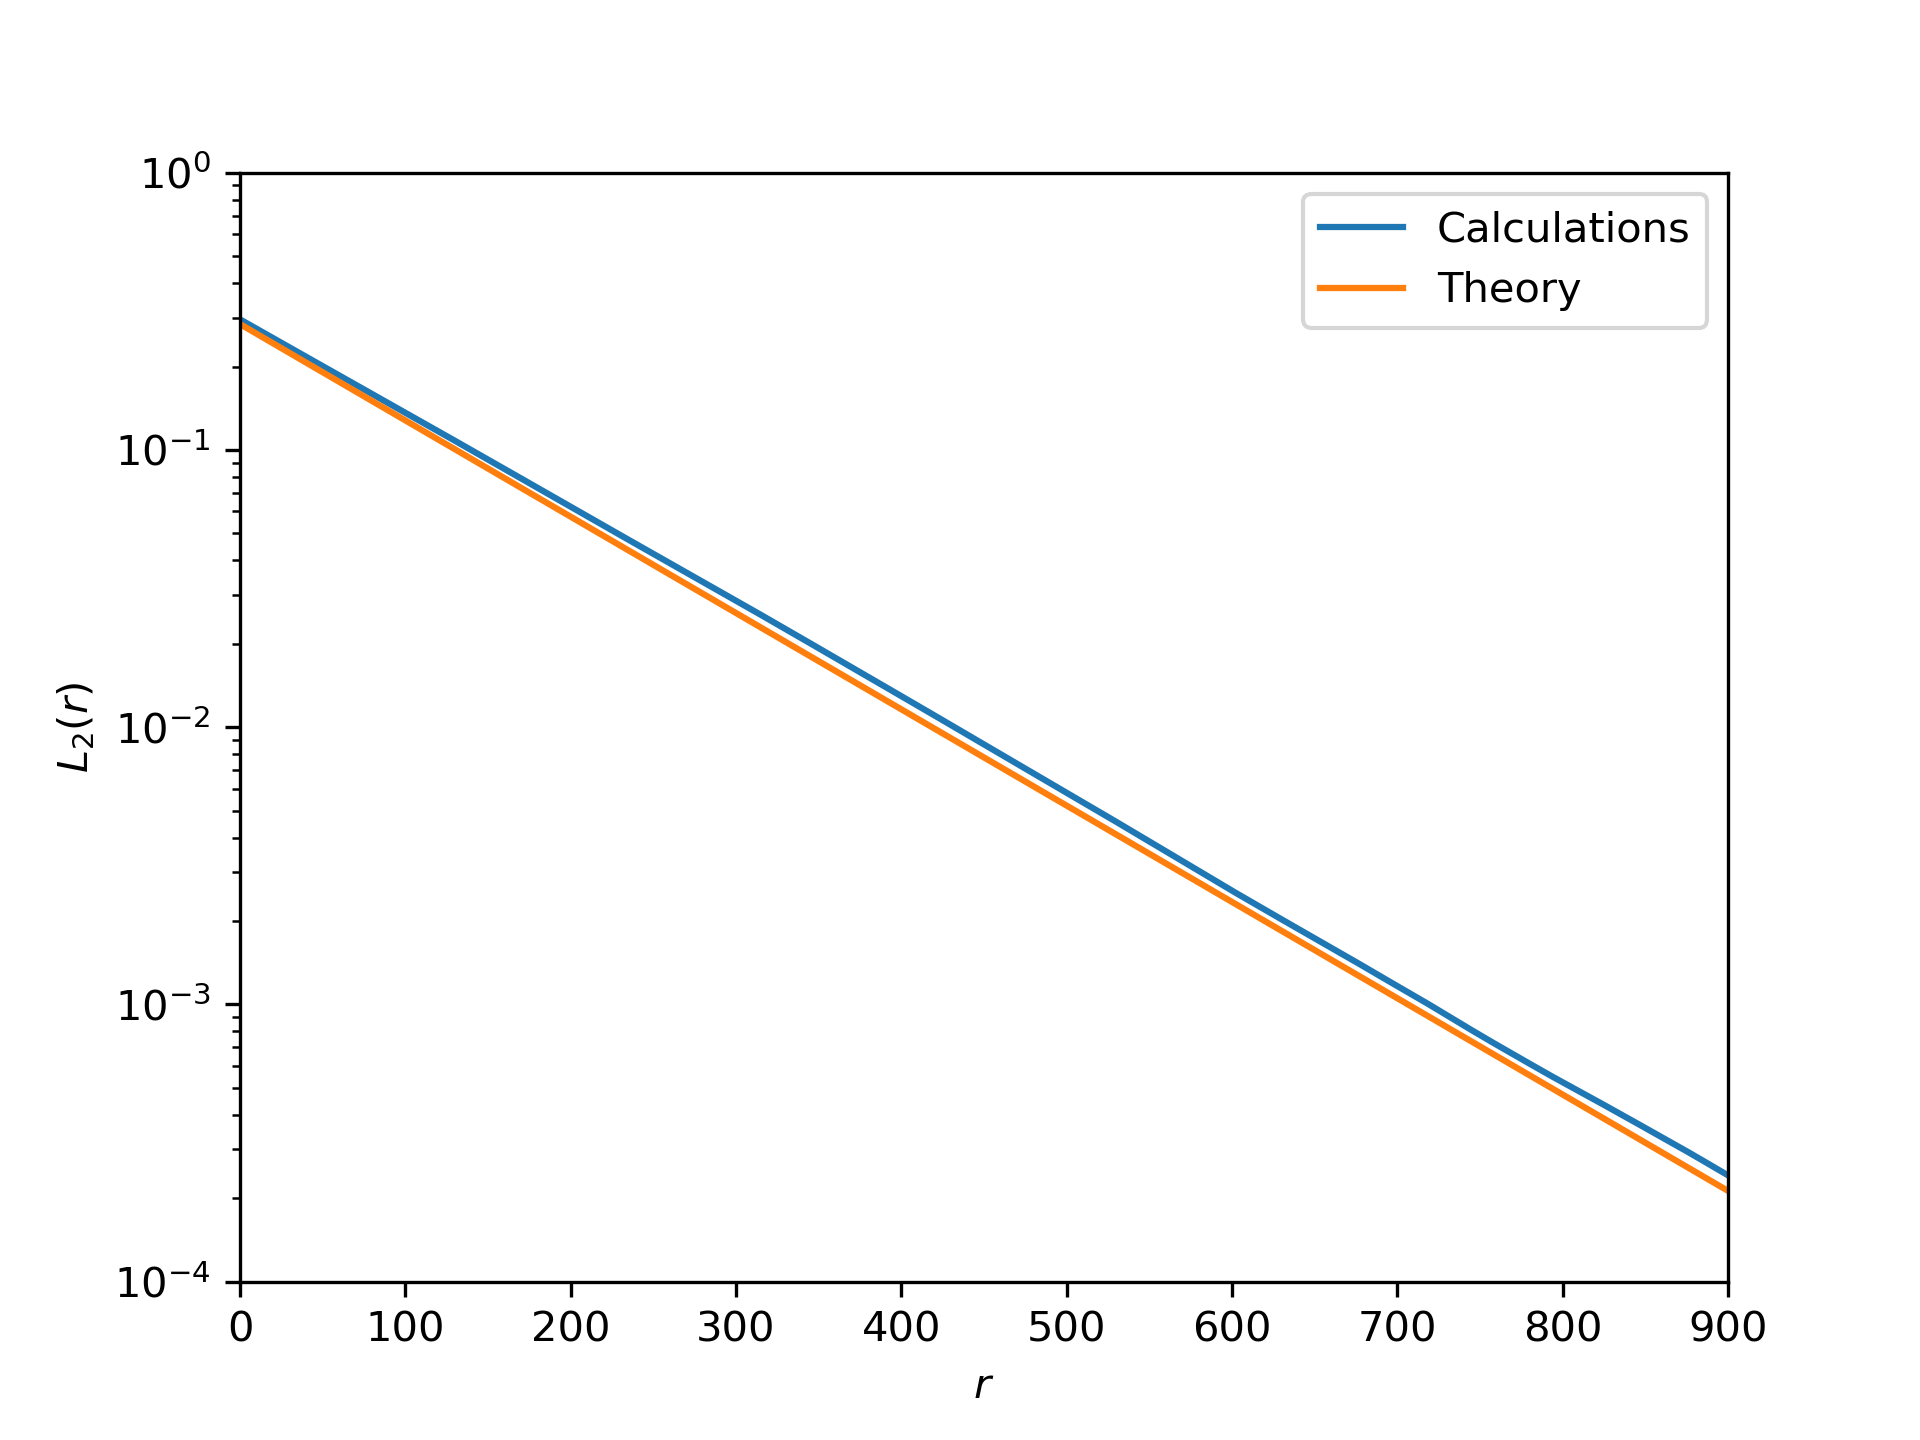
\includegraphics[width=\textwidth]{images/l2-2d.png}
    \caption[]{{\small Lineal-path correlation function}}
    \label{fig:l2-2d}
  \end{subfigure}
  \hfill
  \begin{subfigure}[b]{0.475\textwidth}
    \centering
    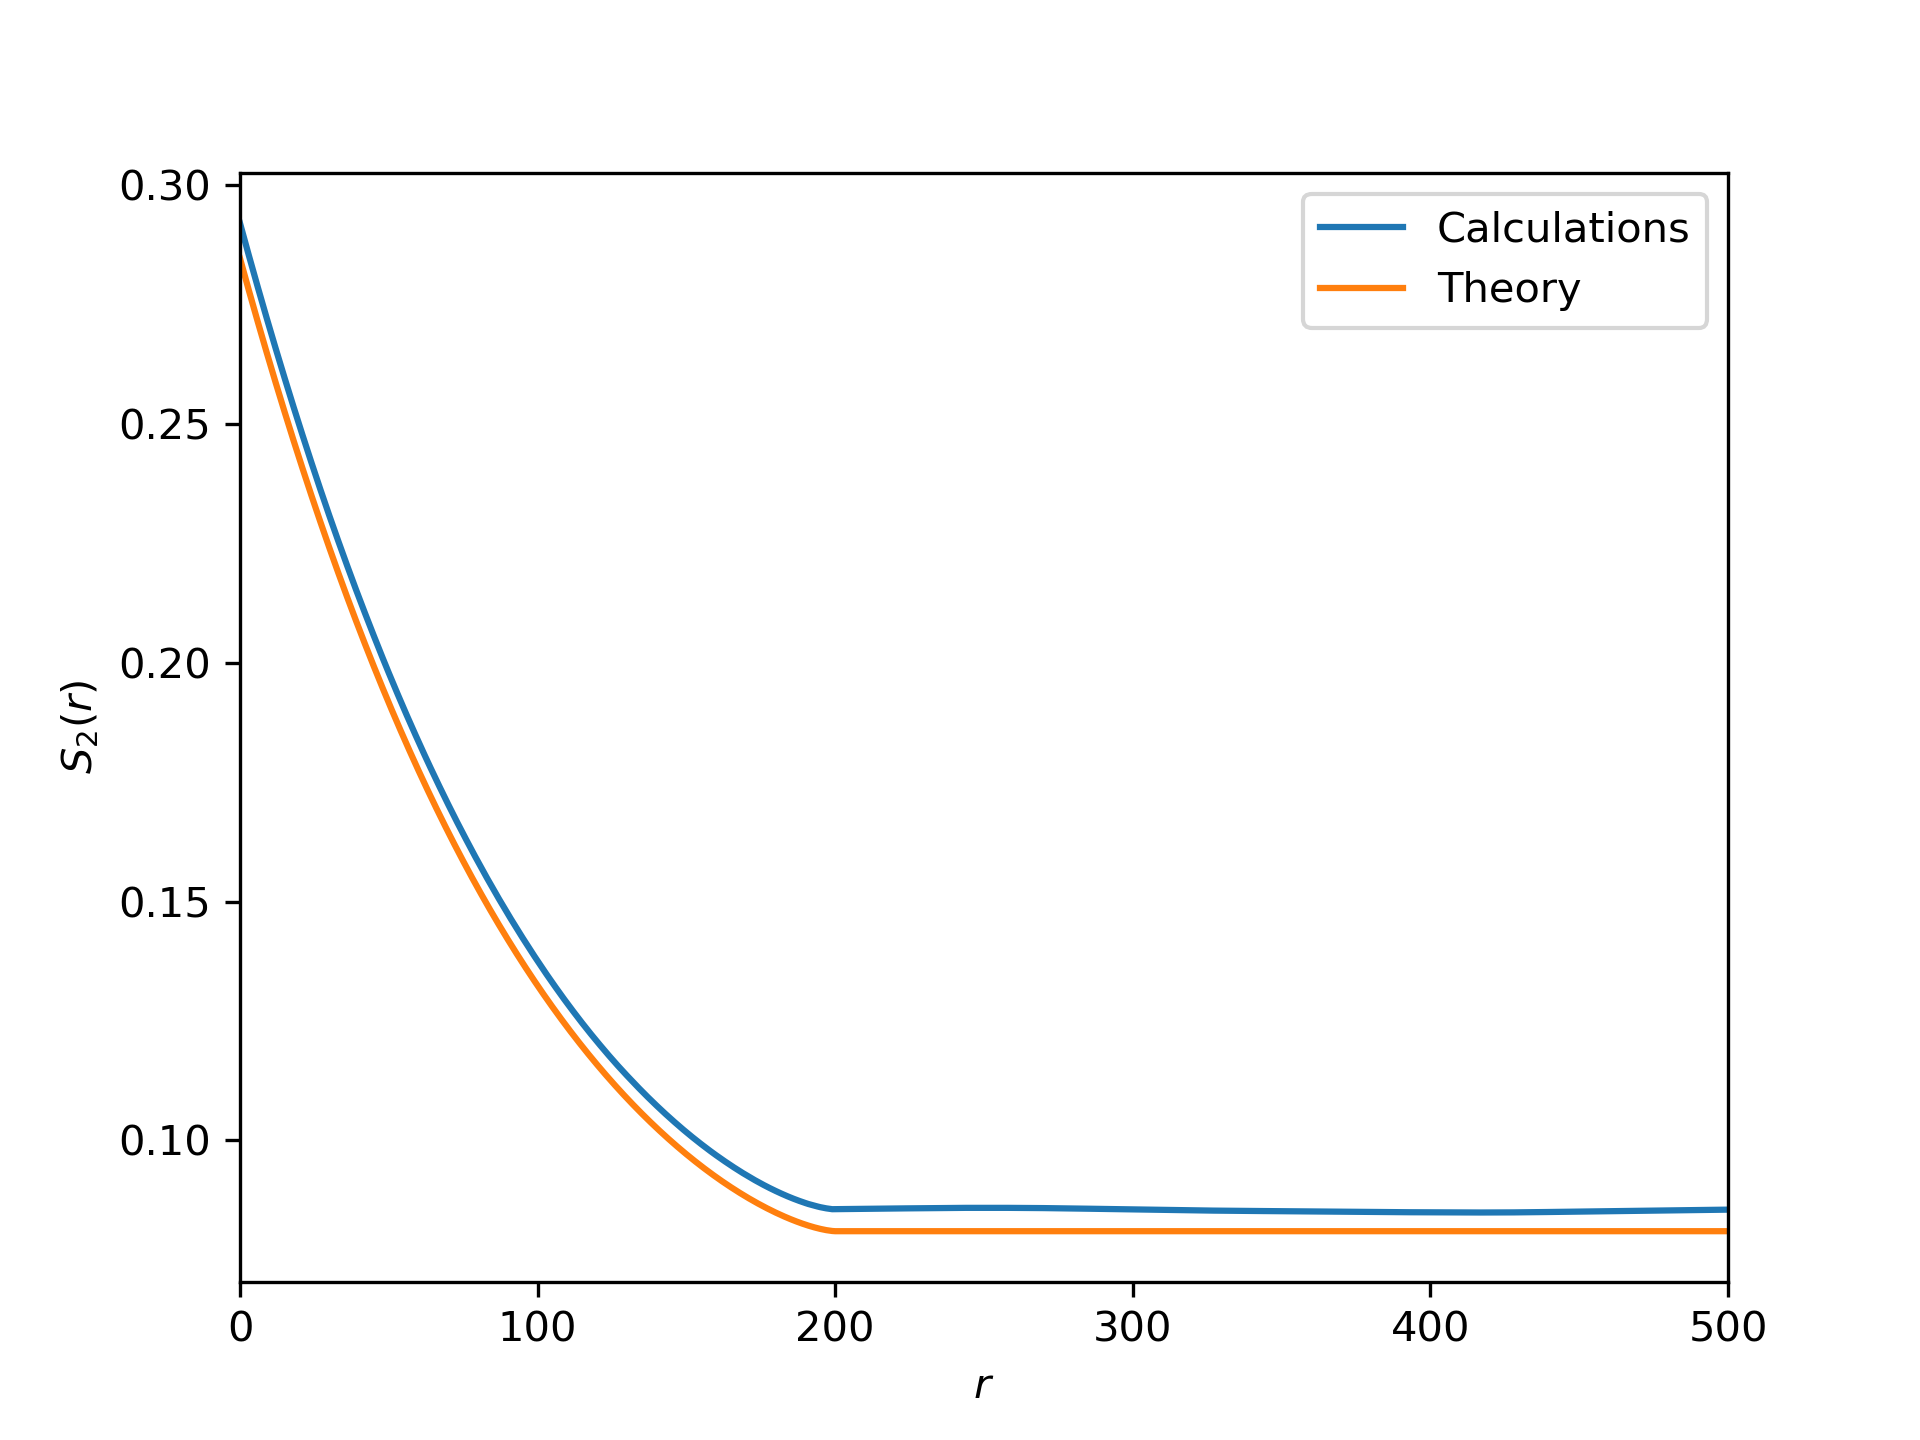
\includegraphics[width=\textwidth]{images/s2-2d.png}
    \caption[]{{\small Two-point correlation function}}
    \label{fig:s2-2d}
  \end{subfigure}
  \vskip\baselineskip
  \begin{subfigure}[b]{0.475\textwidth}
    \centering
    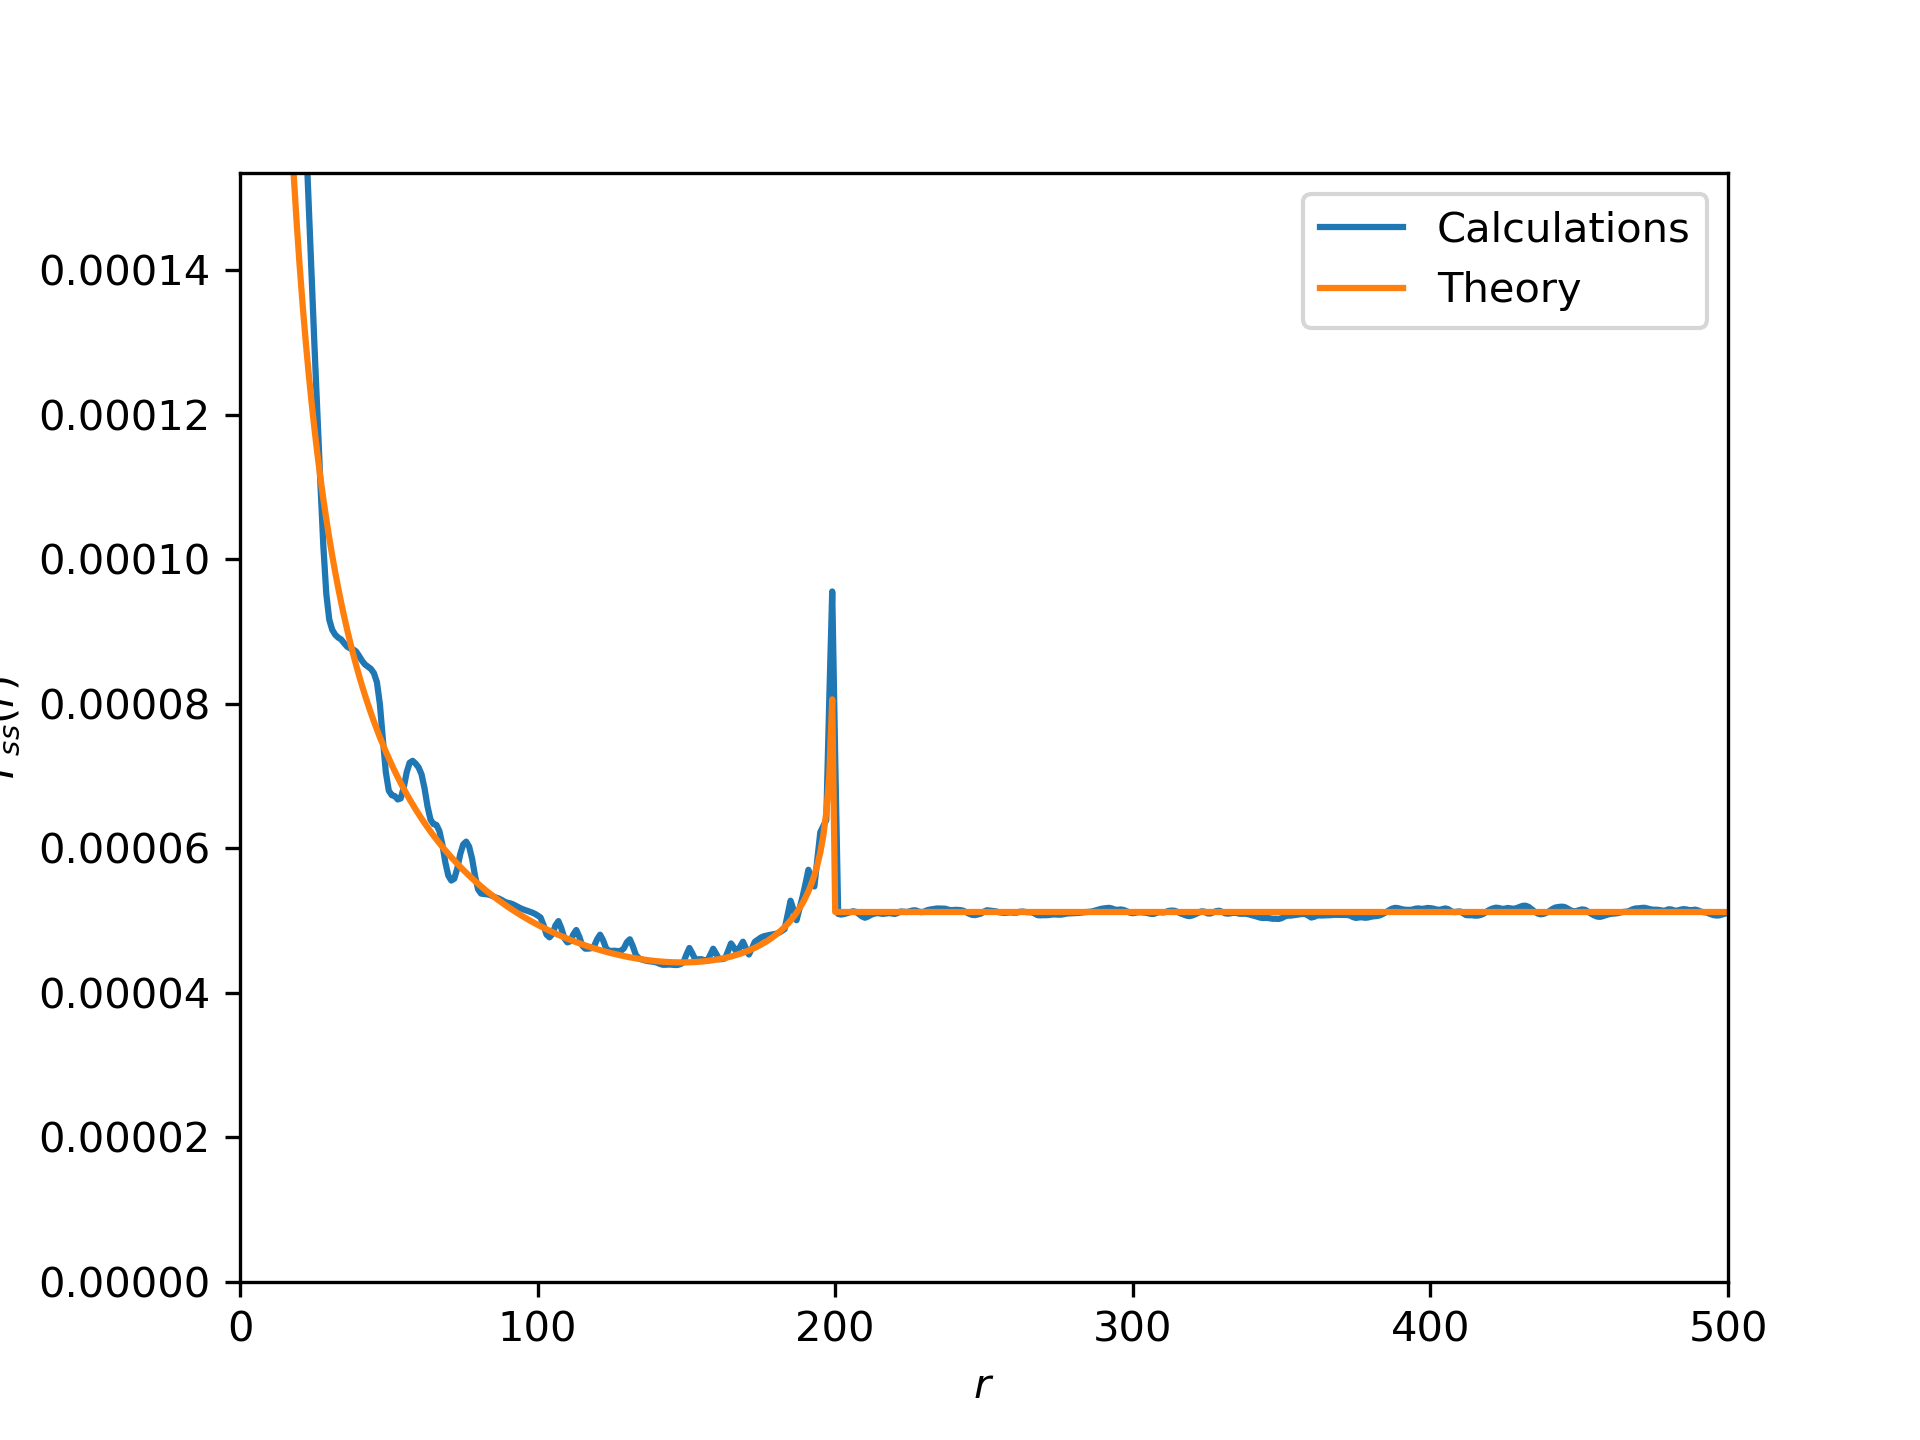
\includegraphics[width=\textwidth]{images/ss-2d.png}
    \caption[]{{\small Surface-surface correlation function}}
    \label{fig:ss-2d}
  \end{subfigure}
  \hfill
  \begin{subfigure}[b]{0.475\textwidth}
    \centering
    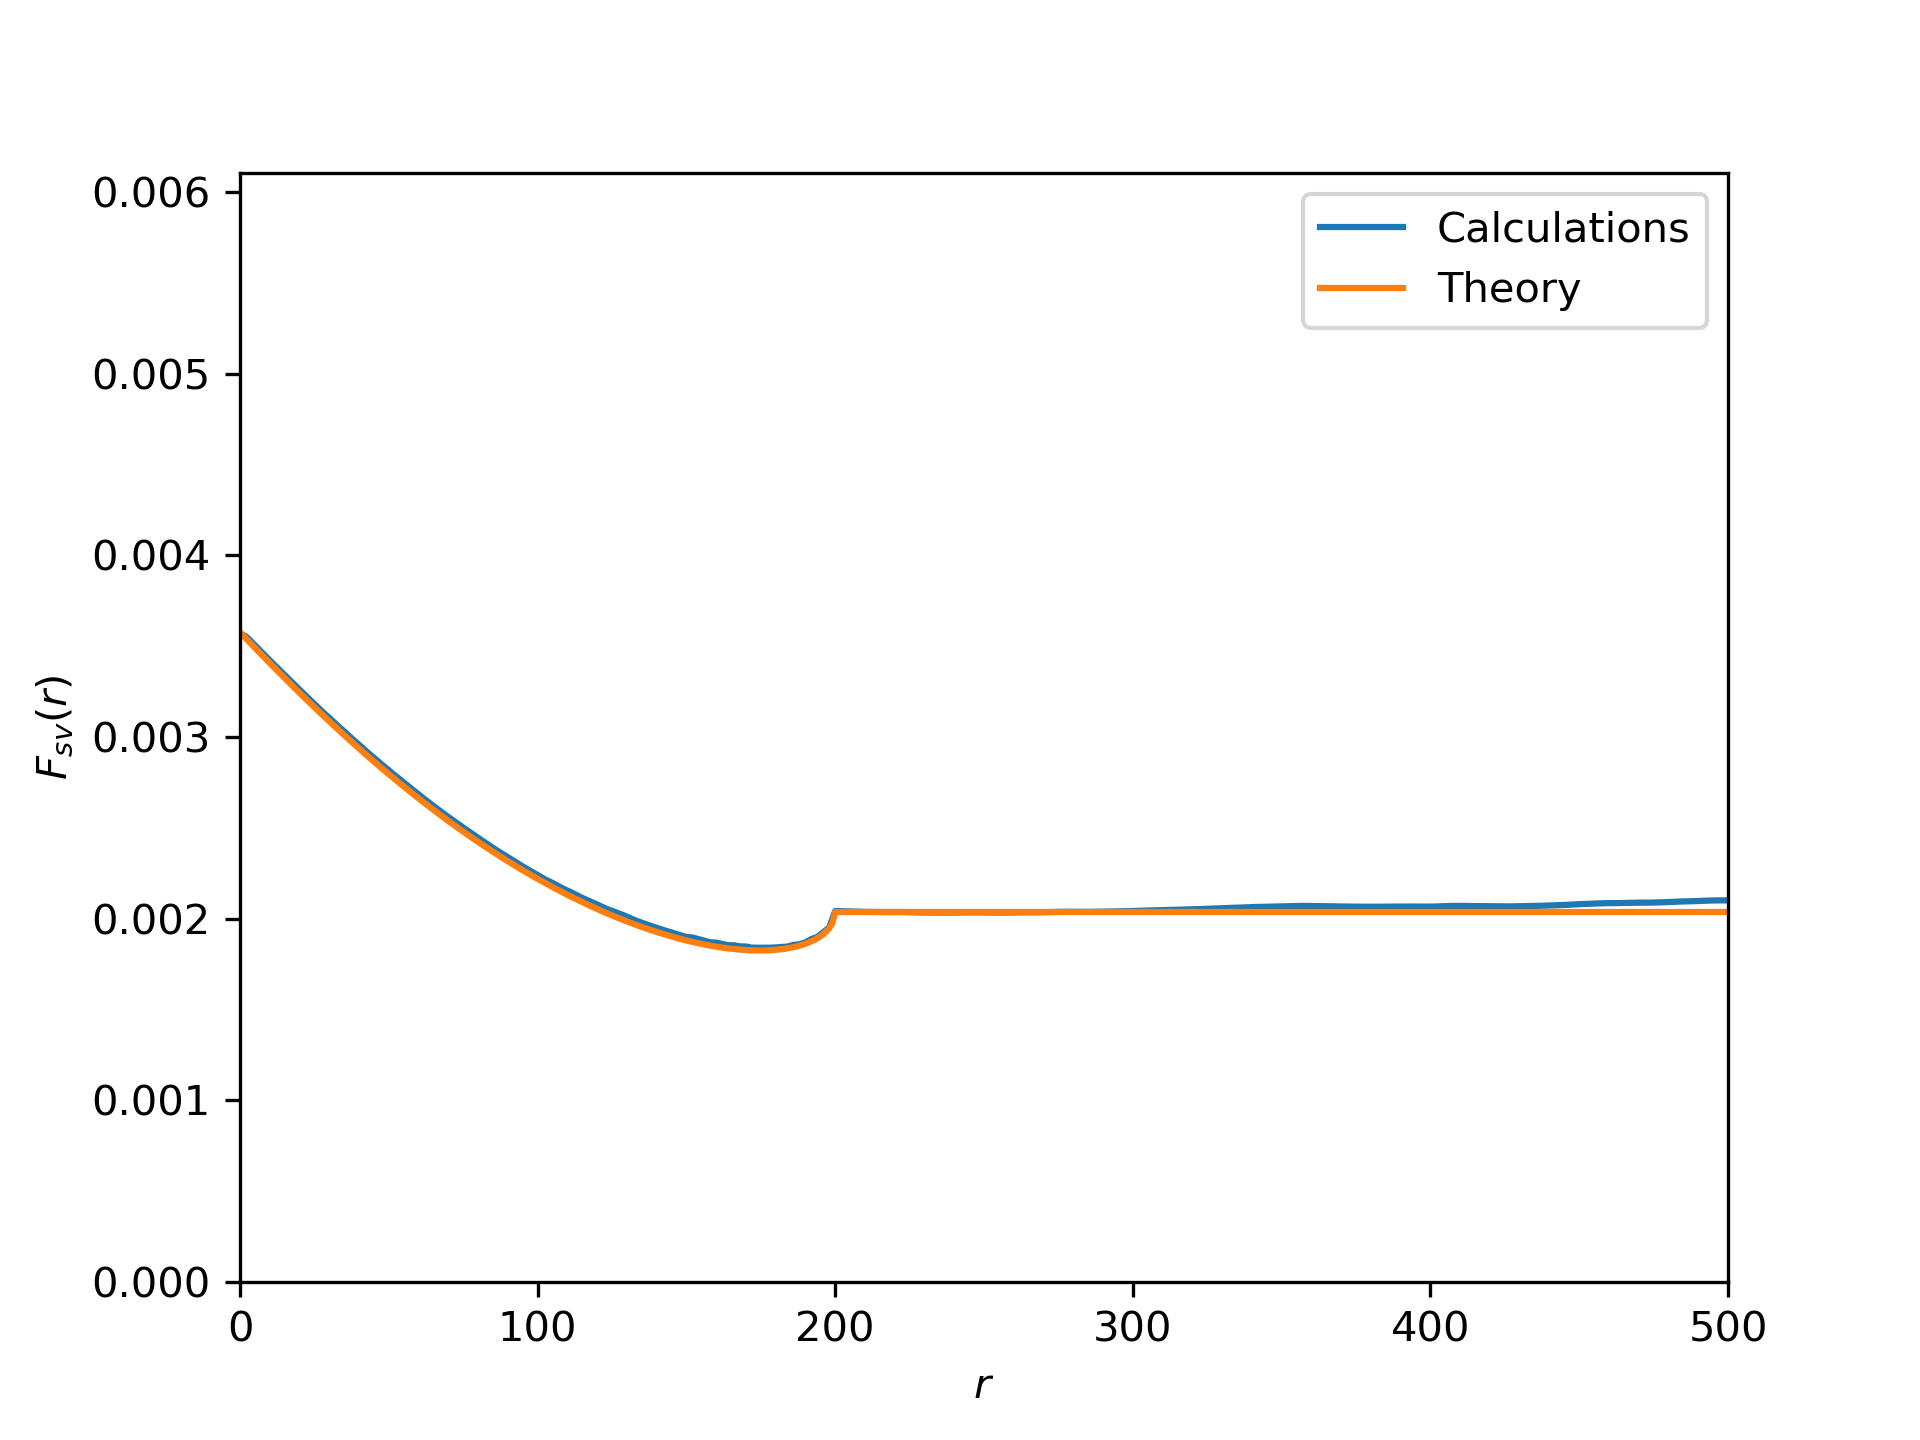
\includegraphics[width=\textwidth]{images/sv-2d.png}
    \caption[]{{\small Surface-void correlation function}}
    \label{fig:sv-2d}
  \end{subfigure}
  \caption[]{\small A comparison of calculated values of $L_2(r)$, $S_2(r)$,
    $F_{ss}(r)$ and $F_{sv}(r)$ with theoretical values for overlapping disks.}
  \label{fig:2d}
\end{figure*}

\begin{figure*}[t]
  \centering
  \begin{subfigure}[b]{0.475\textwidth}
    \centering
    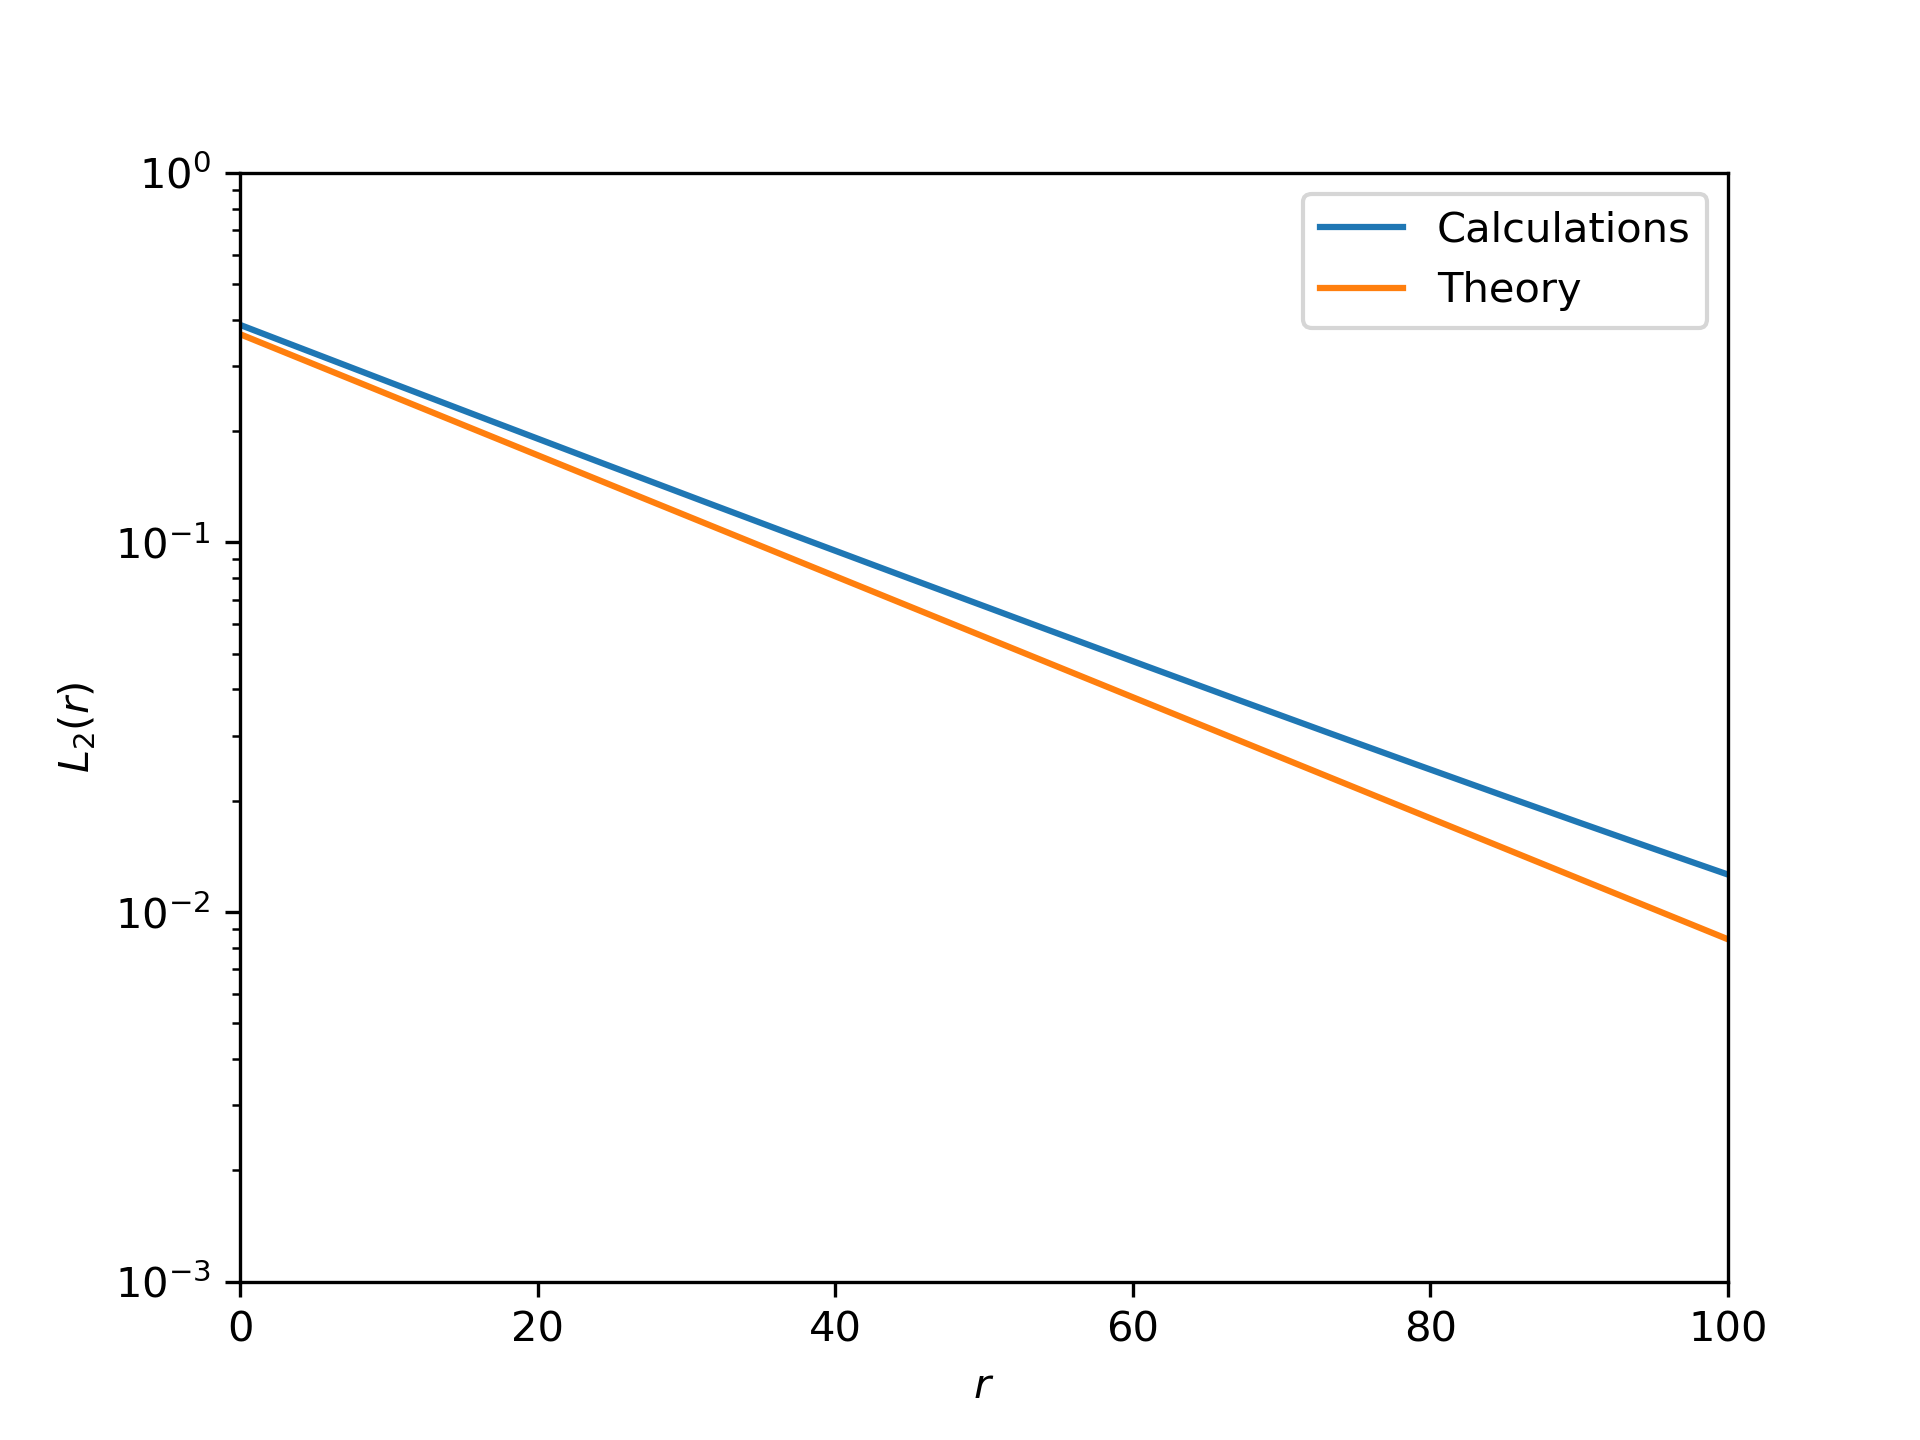
\includegraphics[width=\textwidth]{images/l2-3d.png}
    \caption[]{{\small Lineal-path correlation function}}
    \label{fig:l2-3d}
  \end{subfigure}
  \hfill
  \begin{subfigure}[b]{0.475\textwidth}
    \centering
    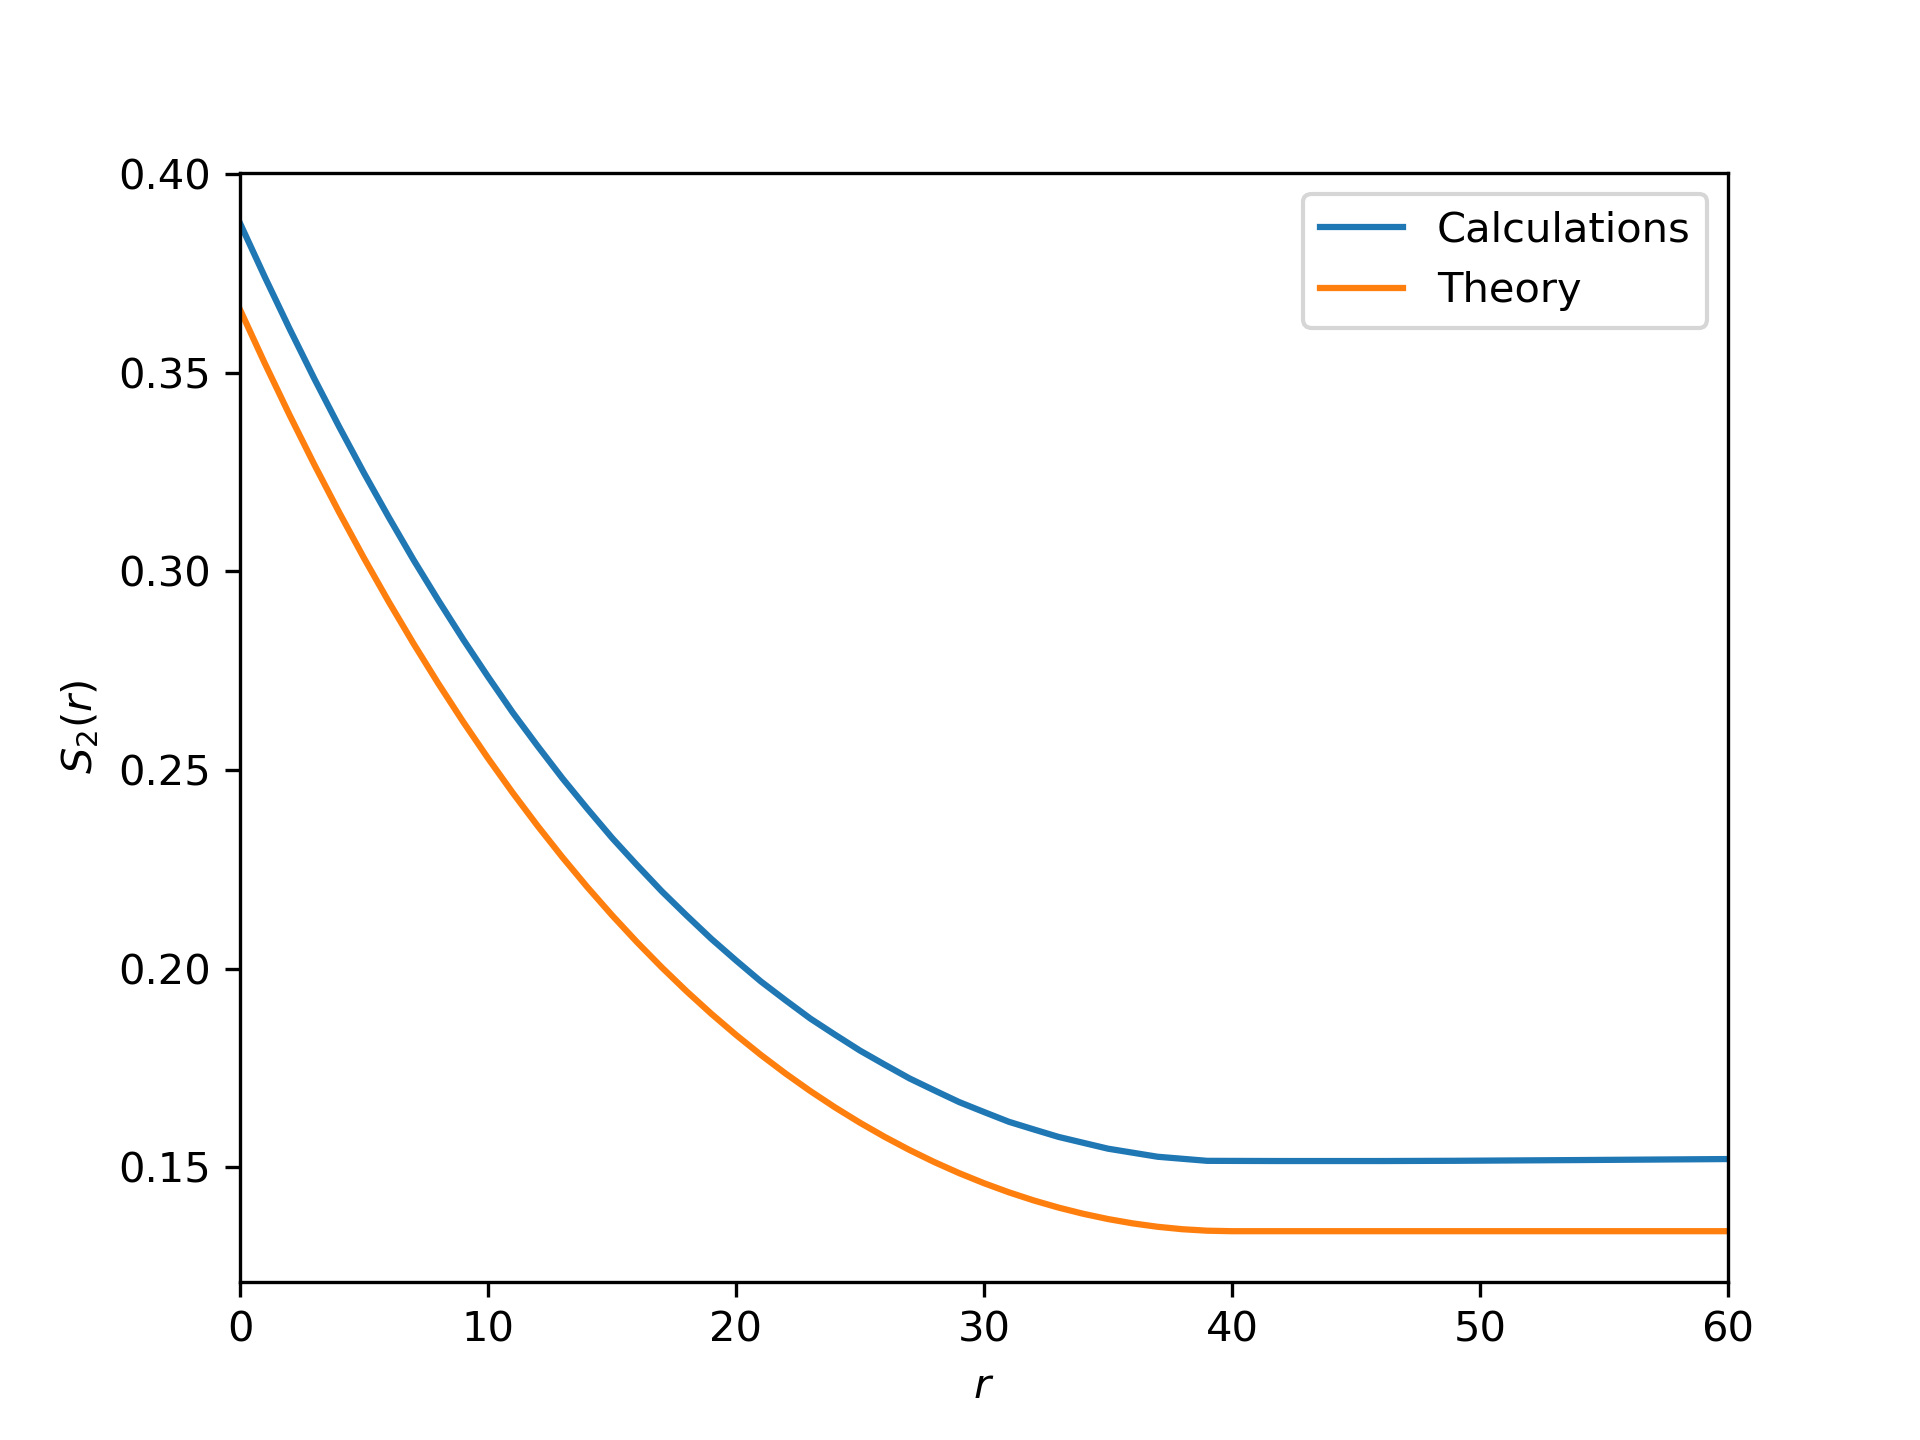
\includegraphics[width=\textwidth]{images/s2-3d.png}
    \caption[]{{\small Two-point correlation function}}
    \label{fig:s3-3d}
  \end{subfigure}
  \vskip\baselineskip
  \begin{subfigure}[b]{0.475\textwidth}
    \centering
    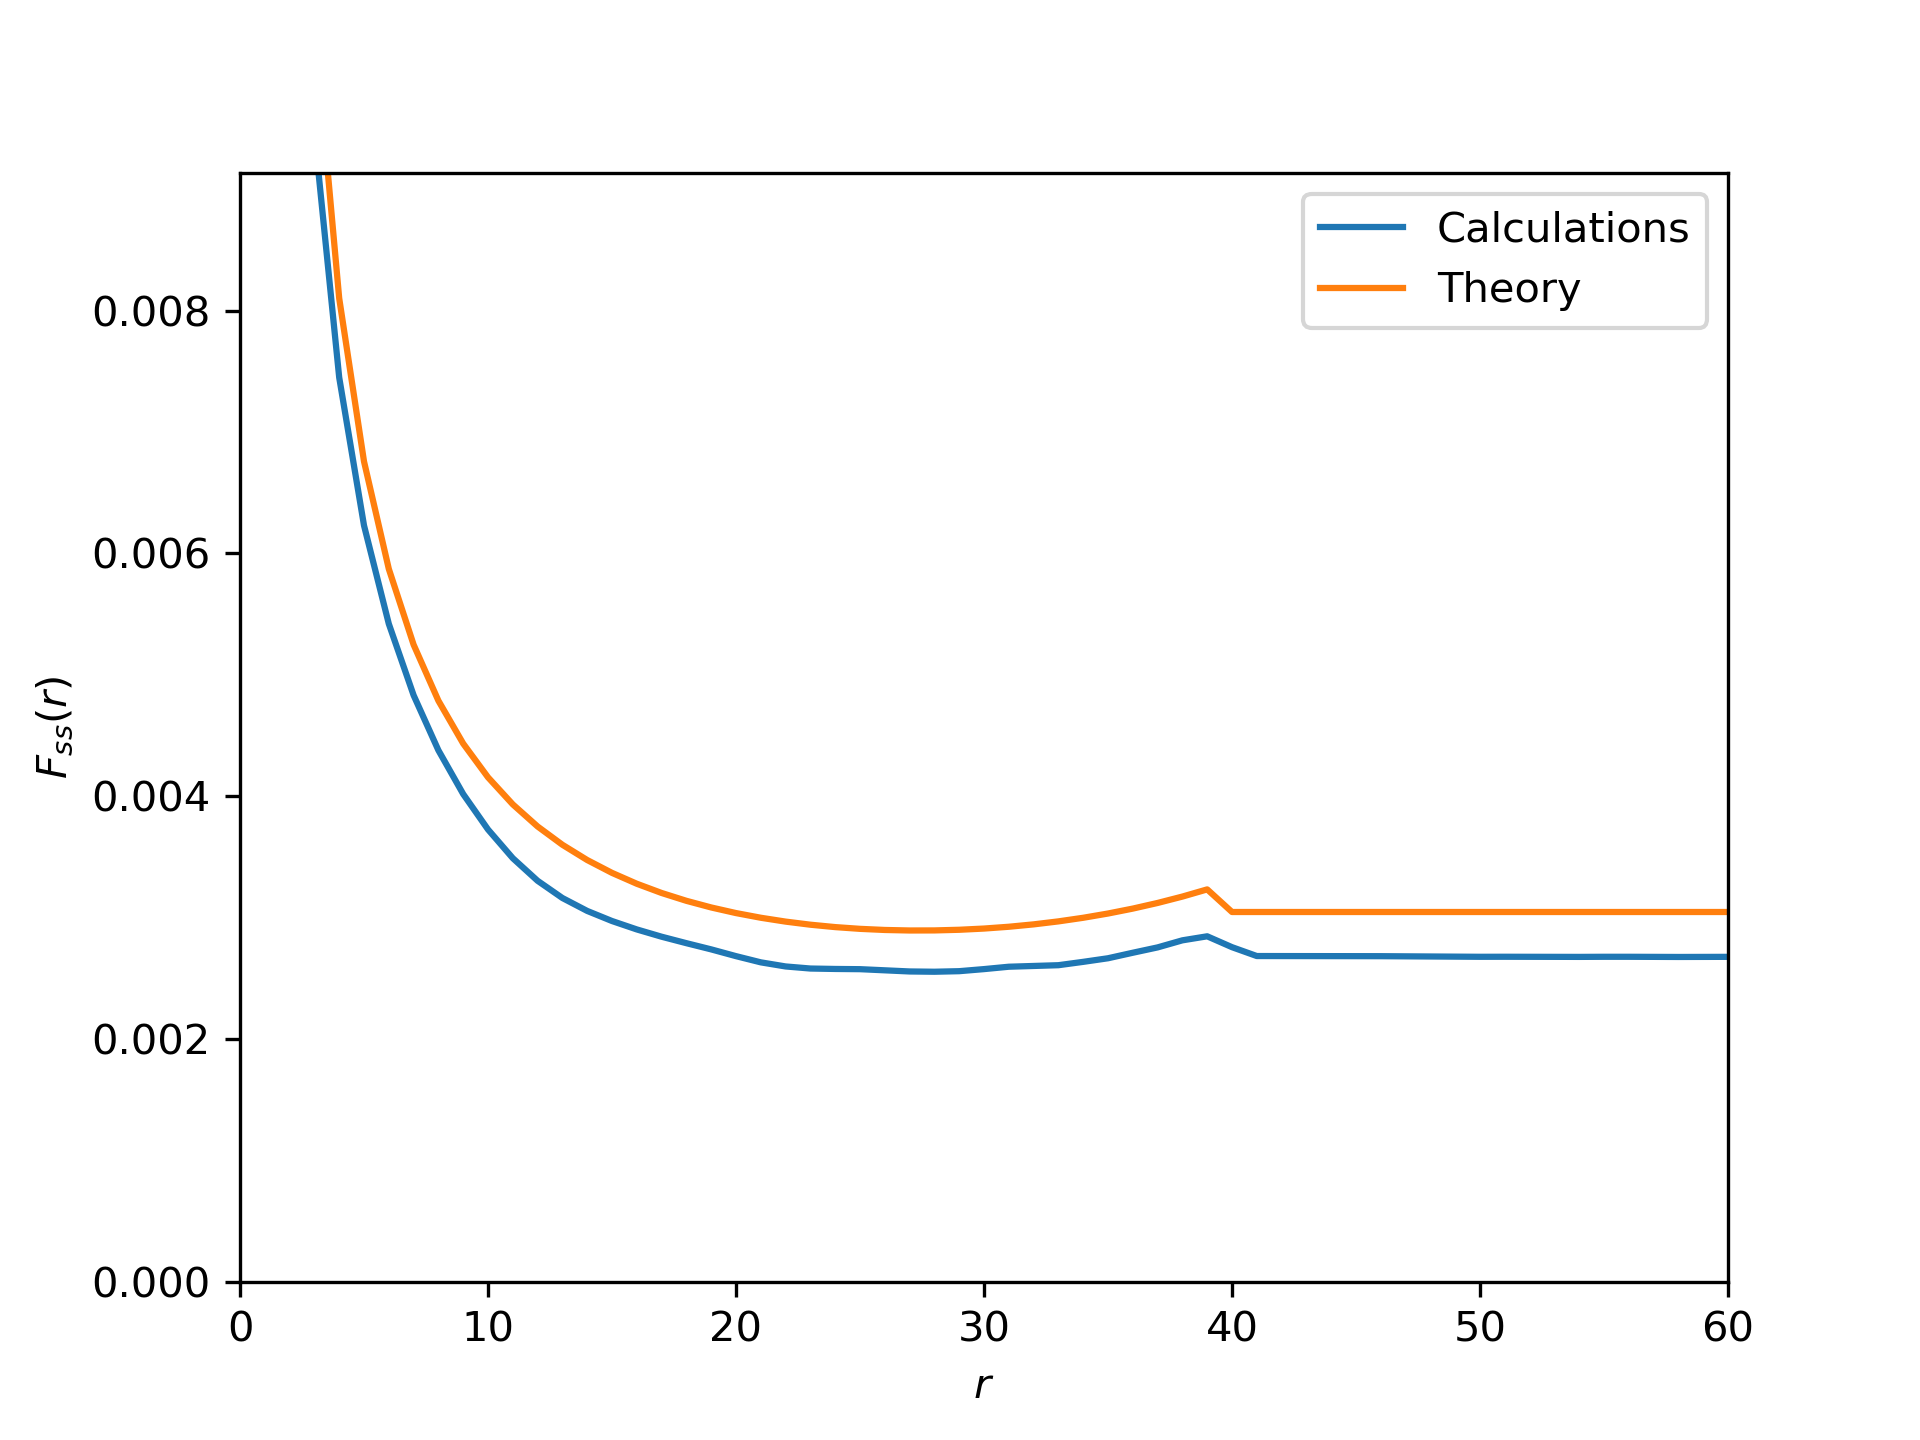
\includegraphics[width=\textwidth]{images/ss-3d.png}
    \caption[]{{\small Surface-surface correlation function}}
    \label{fig:ss-3d}
  \end{subfigure}
  \hfill
  \begin{subfigure}[b]{0.475\textwidth}
    \centering
    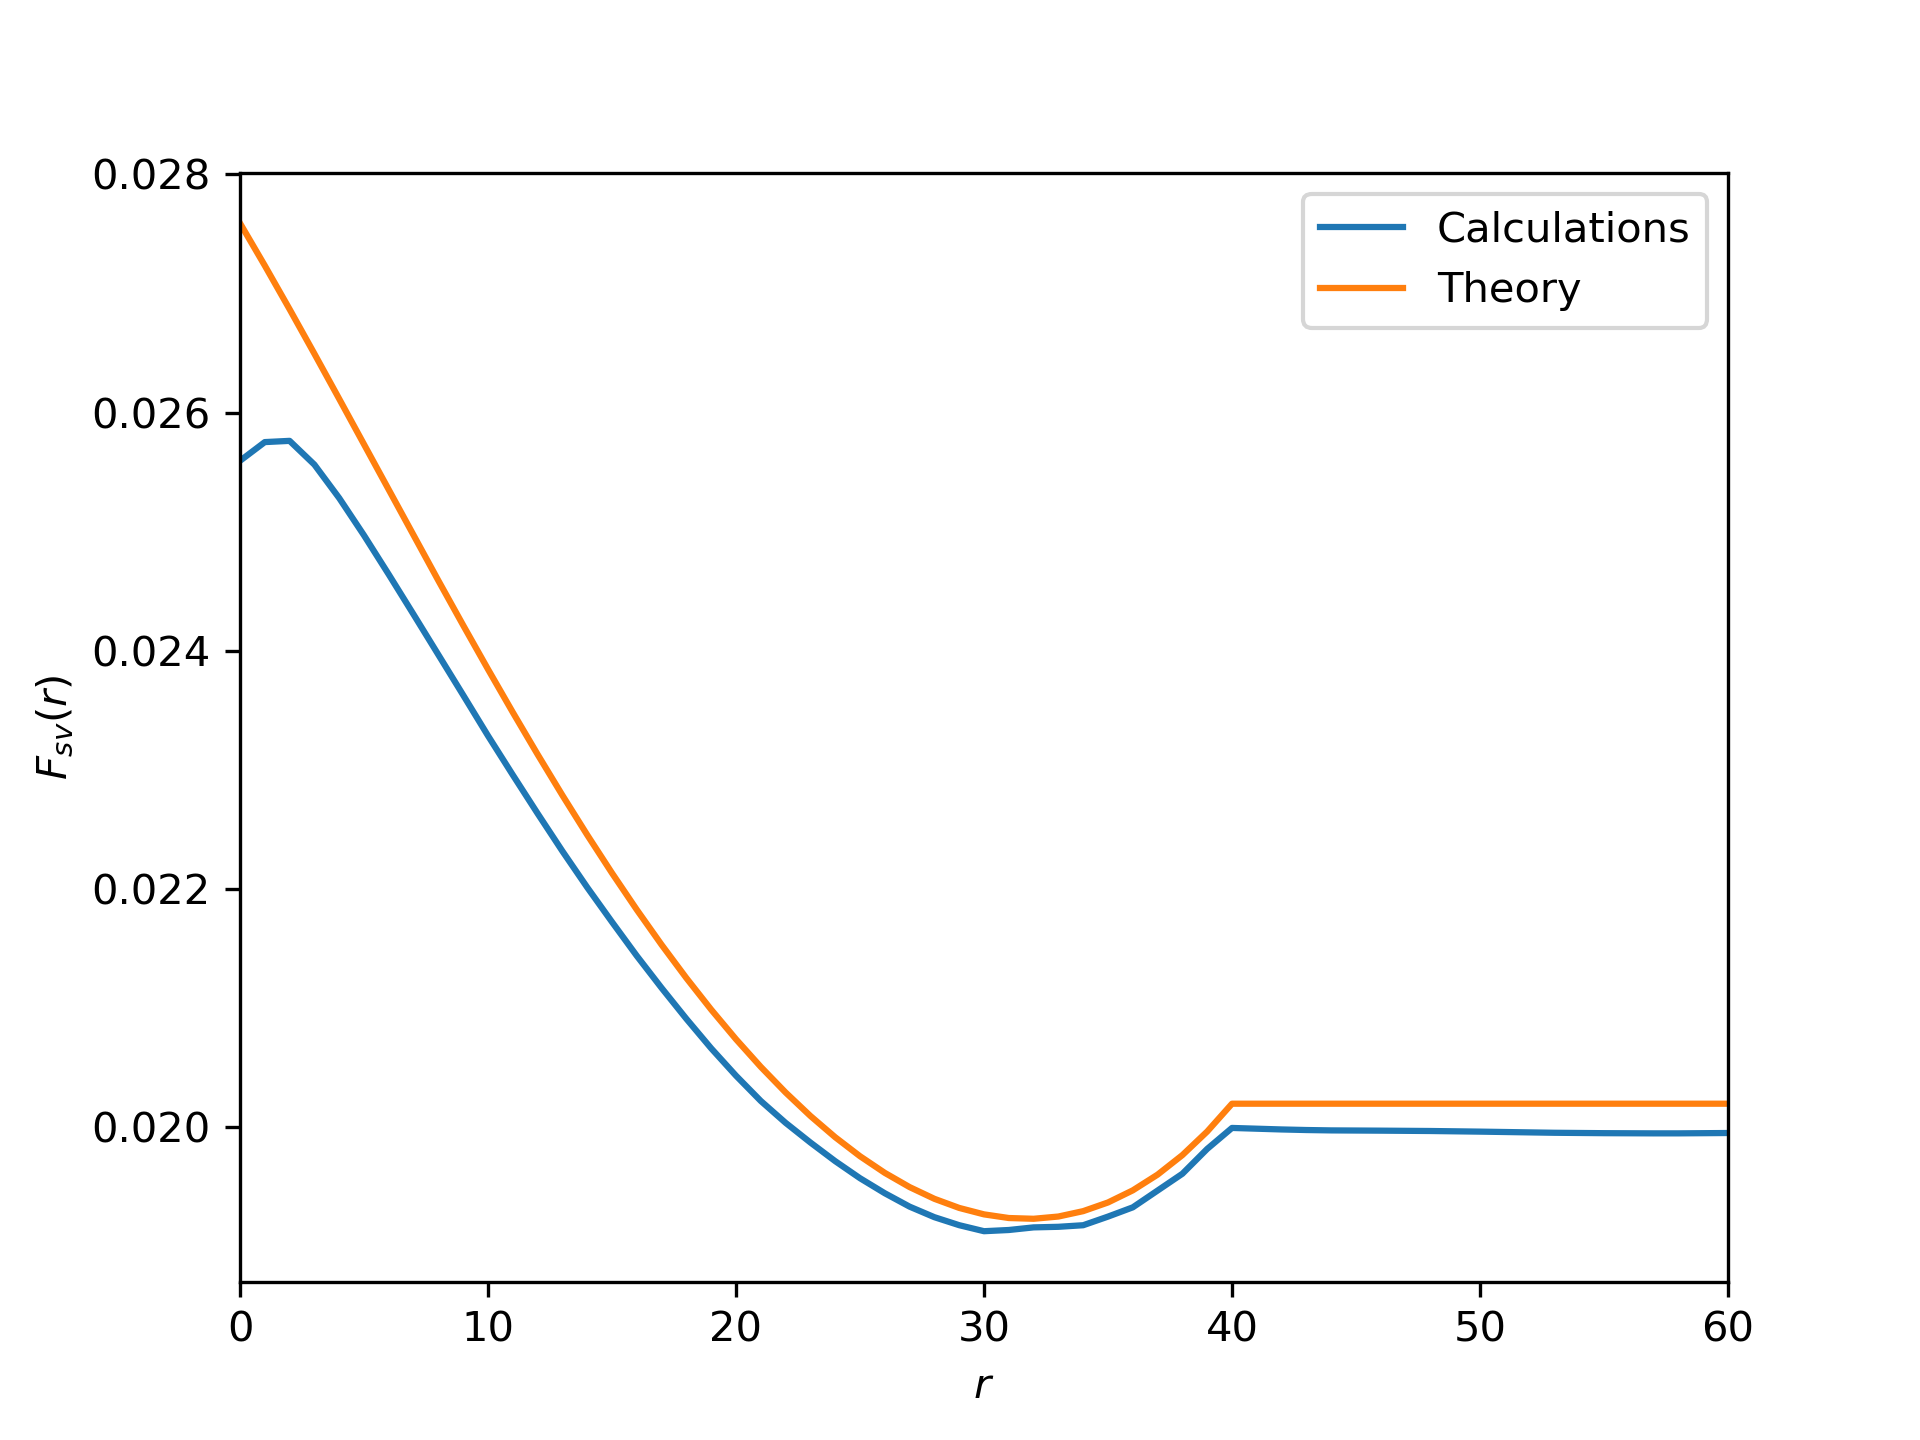
\includegraphics[width=\textwidth]{images/sv-3d.png}
    \caption[]{{\small Surface-void correlation function}}
    \label{fig:sv-3d}
  \end{subfigure}
  \caption[]{\small A comparison of calculated values of $L_2(r)$, $S_2(r)$,
    $F_{ss}(r)$ and $F_{sv}(r)$ with theoretical values for overlapping balls.}
  \label{fig:3d}
\end{figure*}

\begin{figure*}[t]
  \centering
  \begin{subfigure}[b]{0.475\textwidth}
    \centering
    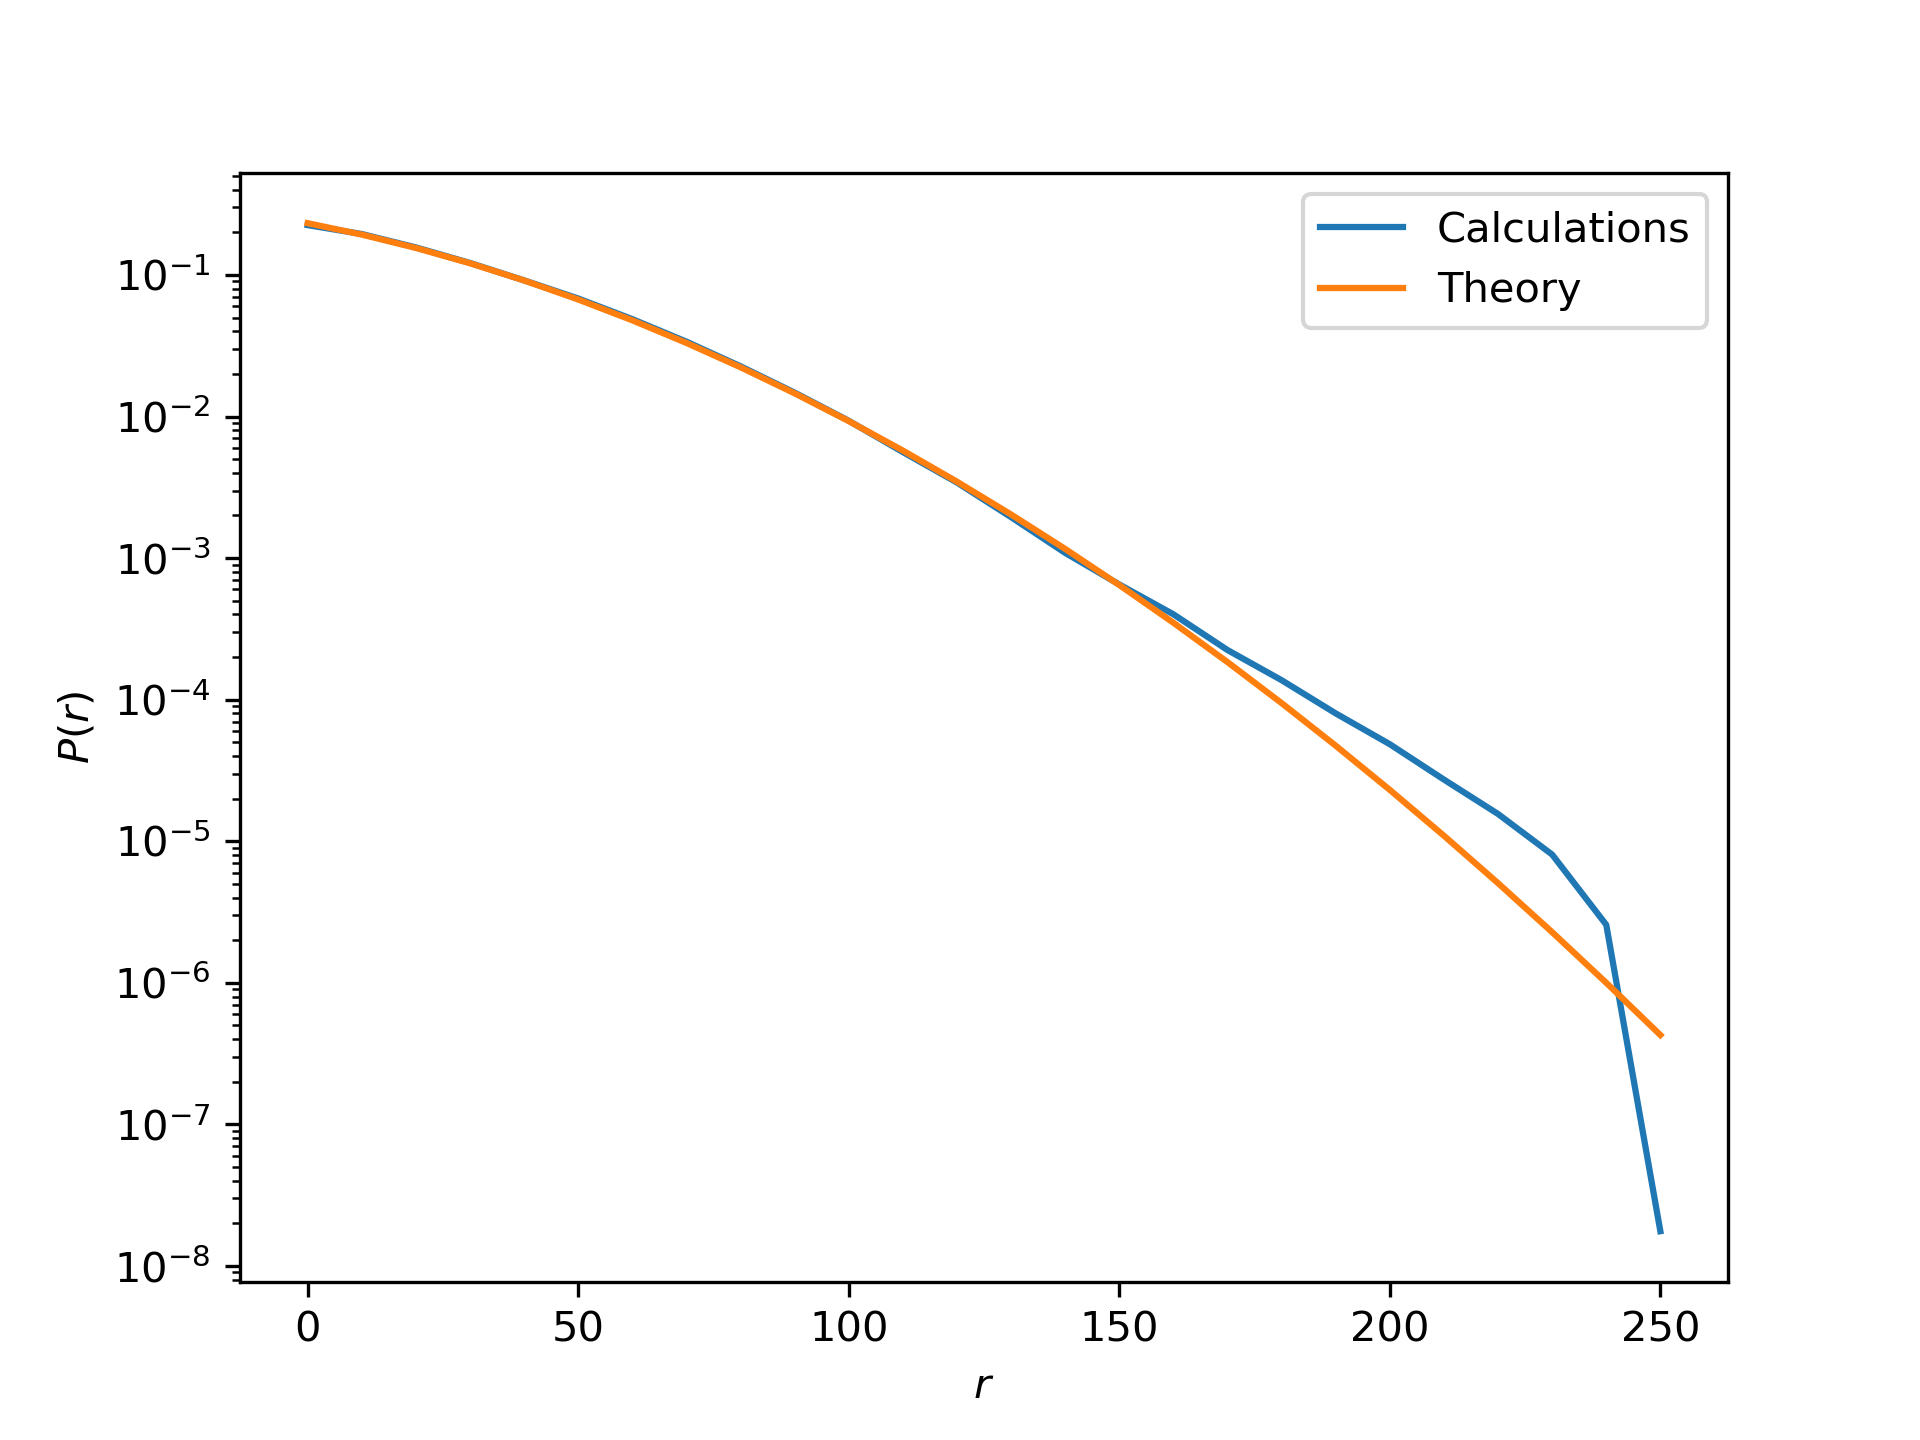
\includegraphics[width=\textwidth]{images/ps-2d.png}
    \caption[]{{\small Pore size correlation function (2D)}}
    \label{fig:ps-2d}
  \end{subfigure}
  \hfill
  \begin{subfigure}[b]{0.475\textwidth}
    \centering
    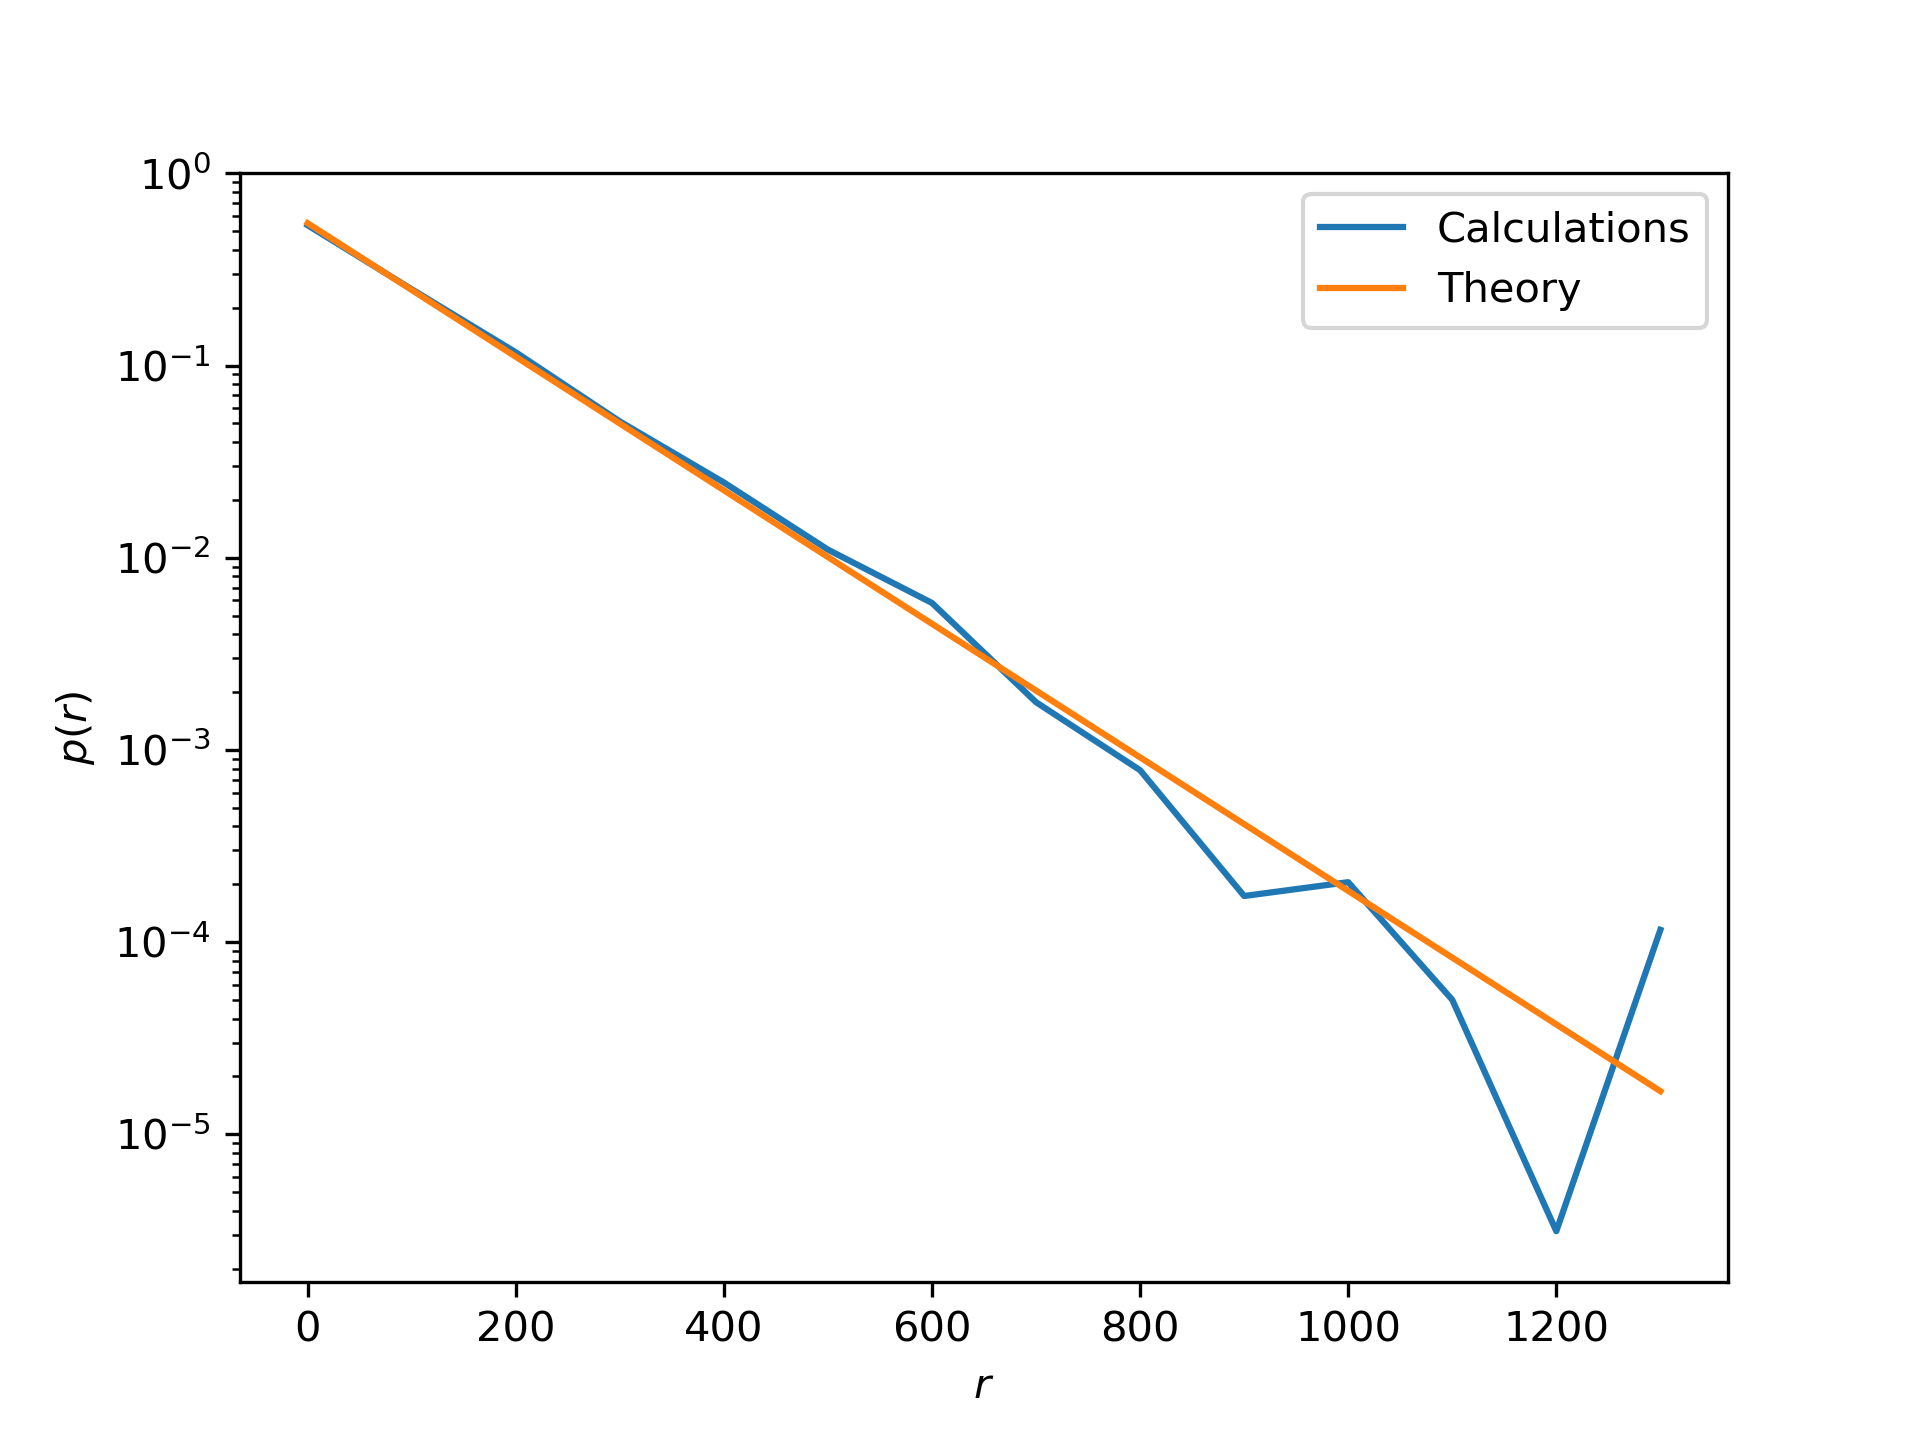
\includegraphics[width=\textwidth]{images/cl-2d.png}
    \caption[]{{\small Chord length correlation function (2D)}}
    \label{fig:cl-2d}
  \end{subfigure}
  \vskip\baselineskip
  \begin{subfigure}[b]{0.475\textwidth}
    \centering
    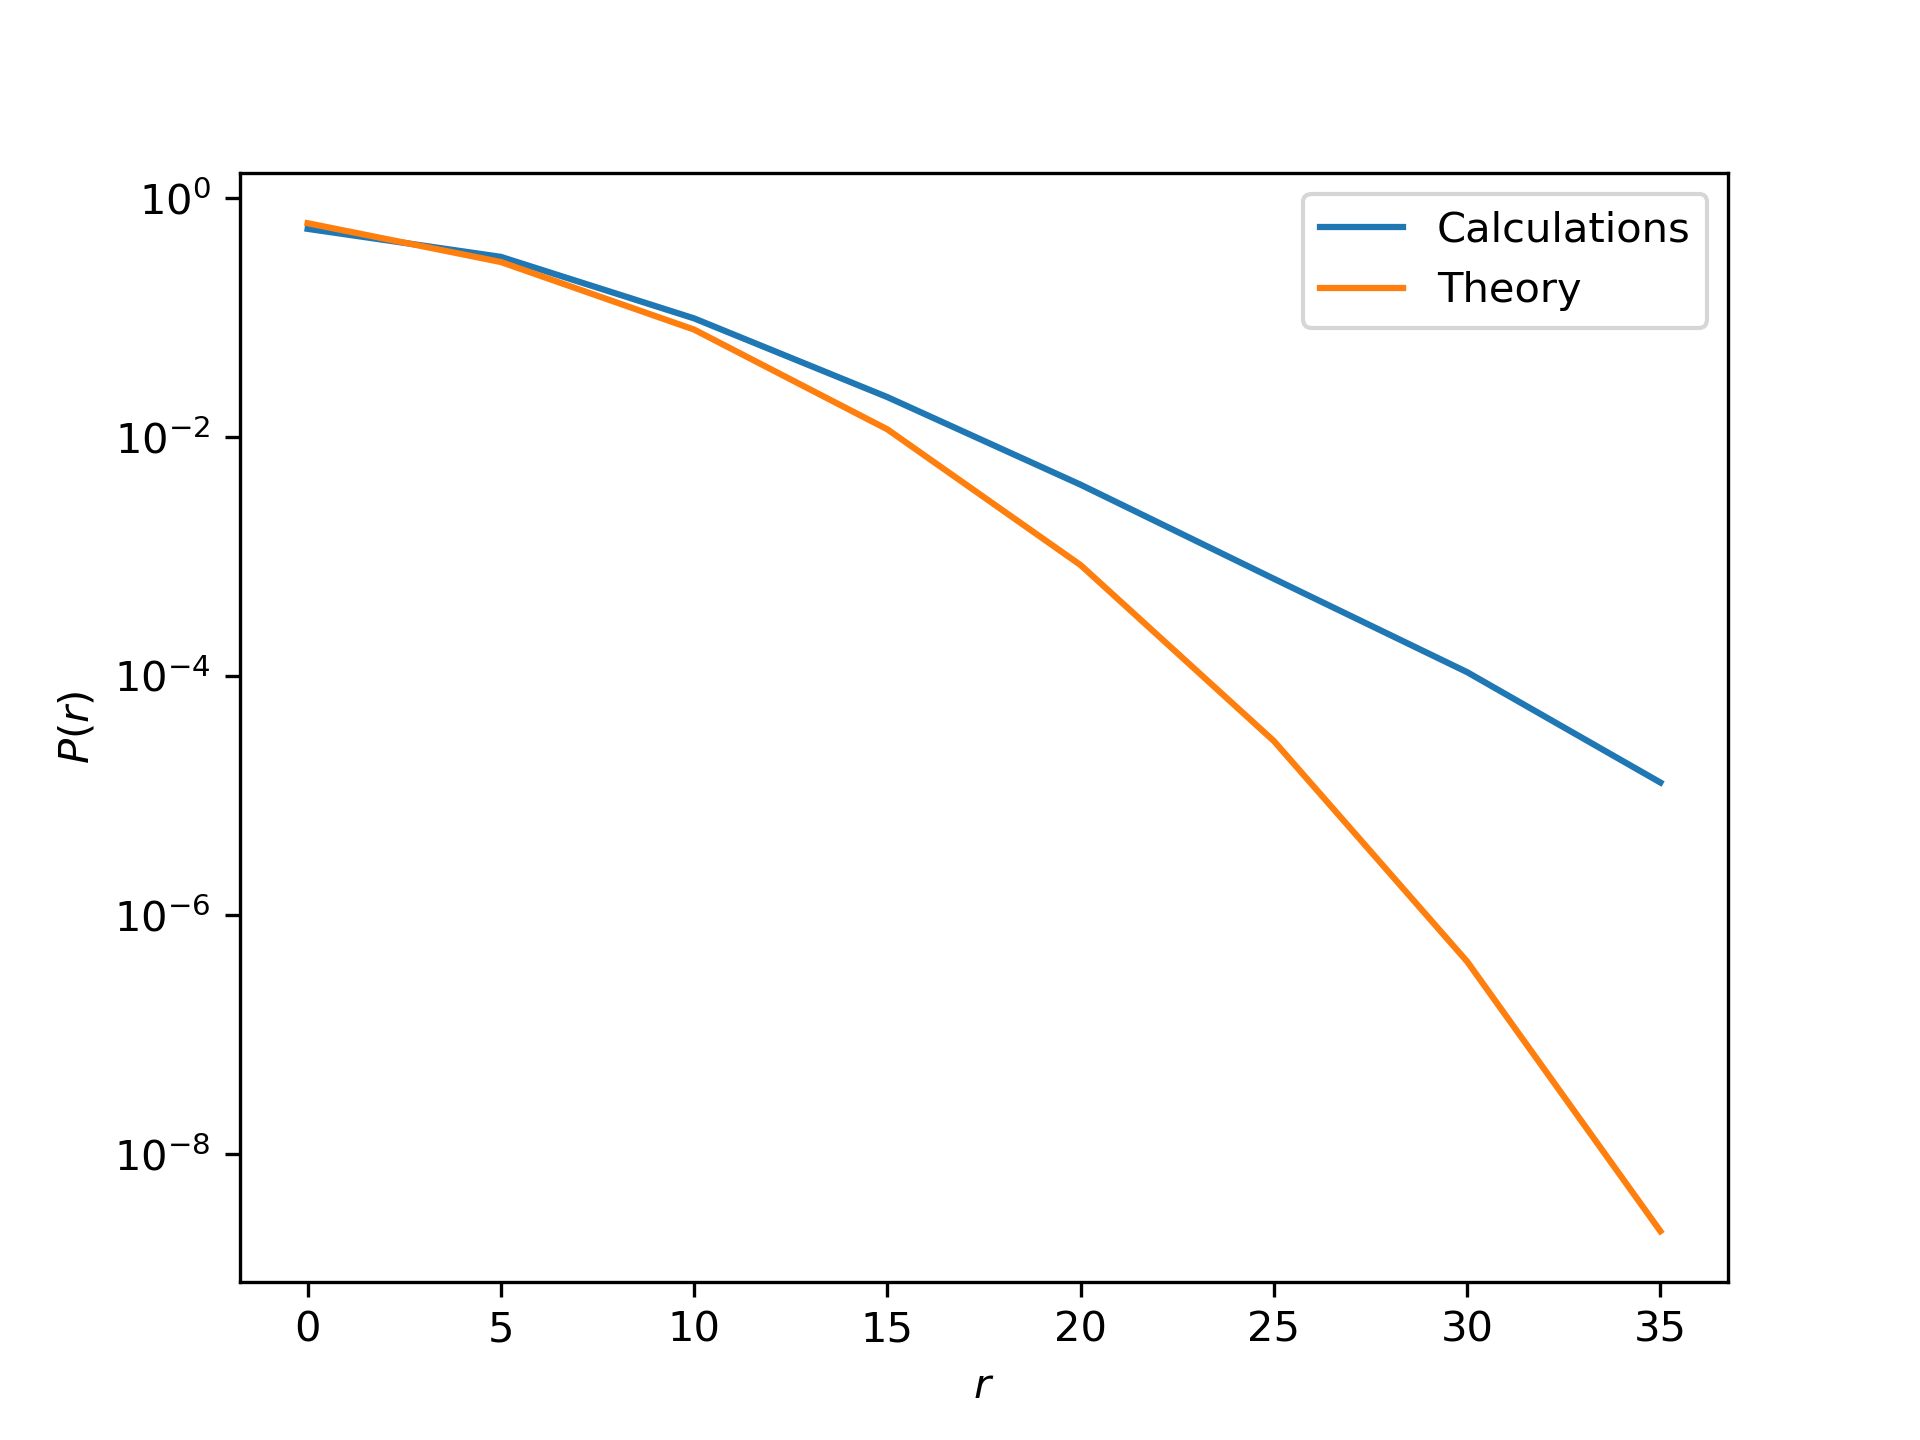
\includegraphics[width=\textwidth]{images/ps-3d.png}
    \caption[]{{\small Pore size correlation function (3D)}}
    \label{fig:ps-3d}
  \end{subfigure}
  \hfill
  \begin{subfigure}[b]{0.475\textwidth}
    \centering
    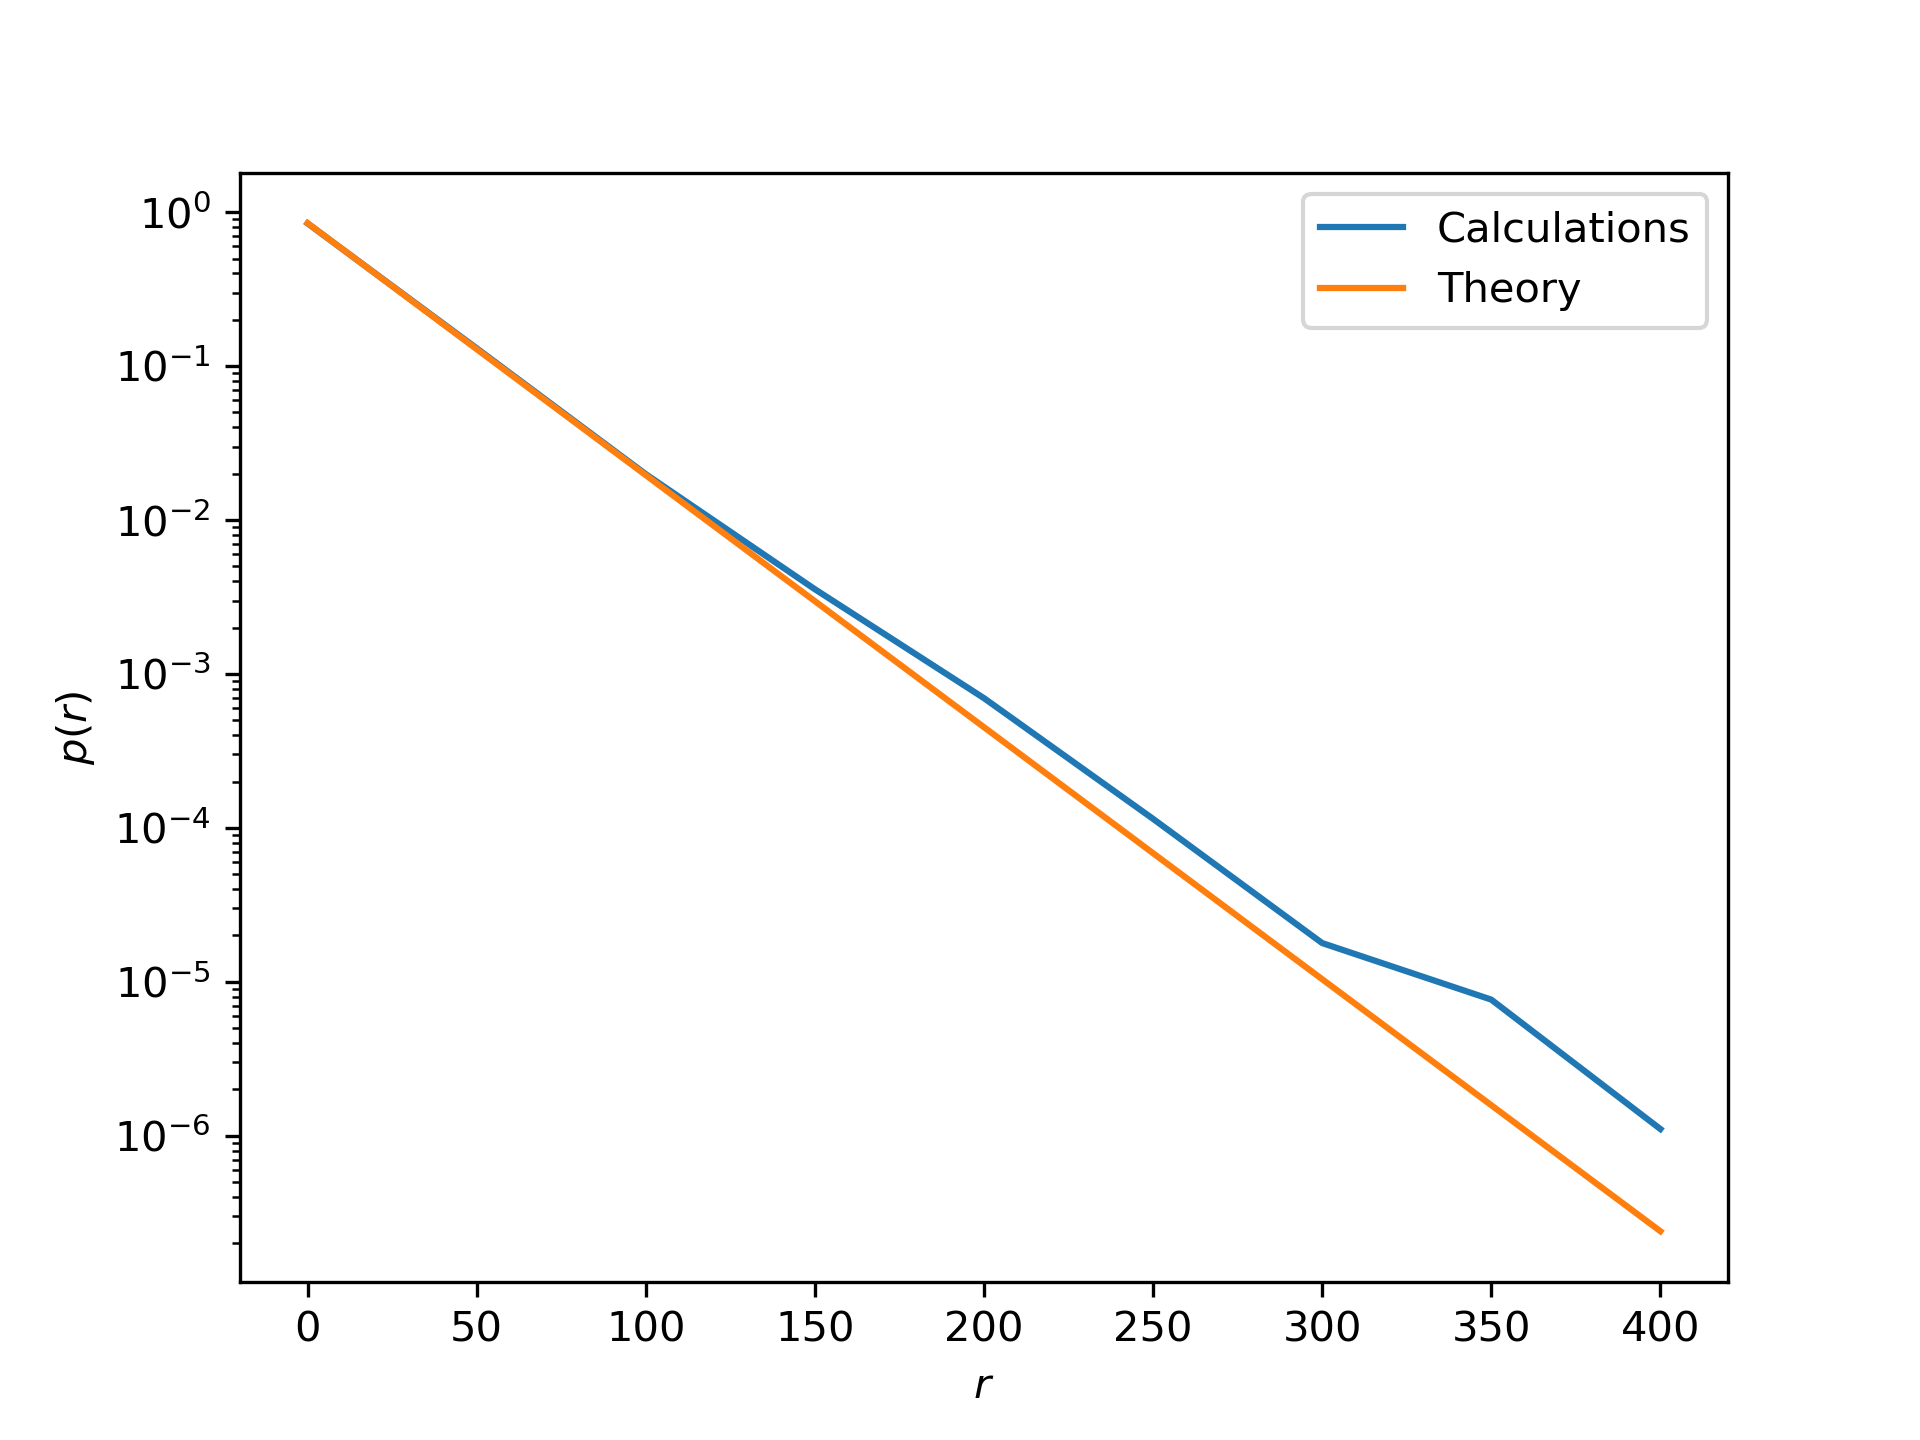
\includegraphics[width=\textwidth]{images/cl-3d.png}
    \caption[]{{\small Chord length correlation function (3D)}}
    \label{fig:cl-3d}
  \end{subfigure}
  \caption[]{\small A comparison of calculated values of $P(r)$ and $p(r)$
    with theoretical values for overlapping disks (\cref{fig:ps-2d} and
    \cref{fig:cl-2d}) and balls(\cref{fig:ps-3d} and \cref{fig:cl-3d}).}
  \label{fig:pscl}
\end{figure*}
\twocolumngrid

\section{Efficiency of our algorithms}

To measure efficiecy of our algorithms we use a machine with the following
configuration:
\begin{itemize}
\item \textbf{CPU}: AMD Ryzen 5 1600X running at 2200~MHz
\item \textbf{Memory}: 32~Gb DDR4-2400 memory
\item \textbf{GPU}: \textbf{Insert nvidia gpu here}
\end{itemize}

We generate two (resp. three) dimensional square (resp. cubic) binary arrays
with different number of elements. The arrays are filled with thresholded value
noise using \code{ValueNoise.jl} package and this code:
\begin{verbatim}
using ValueNoise

getdata(side, dims :: Integer) =
    getdata(side, Val(dims))

getdata(side, :: Val{2}) =
    [value_noise(5x/side,
                 5y/side,
                 0.0,
                 5, 34365) < 0.5
     for x in 1:side, y in 1:side]

getdata(side, :: Val{3}) =
    [value_noise(5x/side,
                 5y/side,
                 5z/side,
                 5, 34365) < 0.5
     for x in 1:side, y in 1:side, z in 1:side]
\end{verbatim}
An example of a two-dimensional image generated in this way is on
\cref{fig:valuenoise}. The function \code{getdata} generates the same image
sampled with different resolutions.

To measure efficiency of \code{Directional} module we generate ten arrays with
a side of a square $s = 1000, 2000, \dots, 10000$ pixels for two-dimensional
case and ten arrays with a side of a cube $s = 50, 100, \dots, 500$ voxels for
three-dimensional case and calculate execution time for each function. All
functions are calculated with default values of optional arguments (that is:
closed walls boundary conditions and computation along axial directions).

To measure efficiency of \code{Map} module we follow the same procedure but with
seven arrays usings squares with a side $s = 1000, 2000, \dots, 7000$ pixels and
cubes with a side $s = 50, 100, \dots, 350$ voxels.

The measurements of execution time is on \cref{fig:timings}.

\begin{figure}[ht]
  \centering
  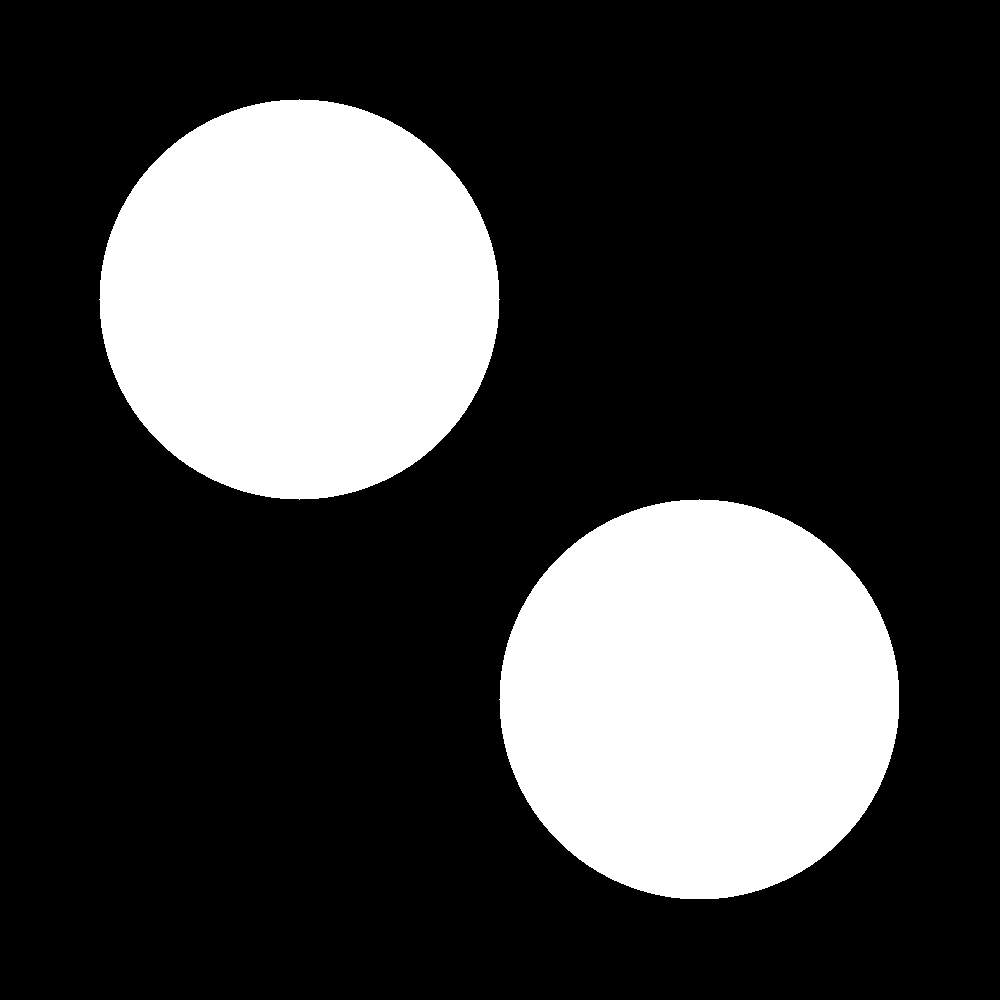
\includegraphics[width=.3\textwidth]{images/timing-image.png}
  \caption[]{{\small An example of 2D image used in timing measurements}}
  \label{fig:valuenoise}
\end{figure}

\onecolumngrid
\begin{figure*}[t]
  \centering
  \begin{subfigure}[b]{0.475\textwidth}
    \centering
    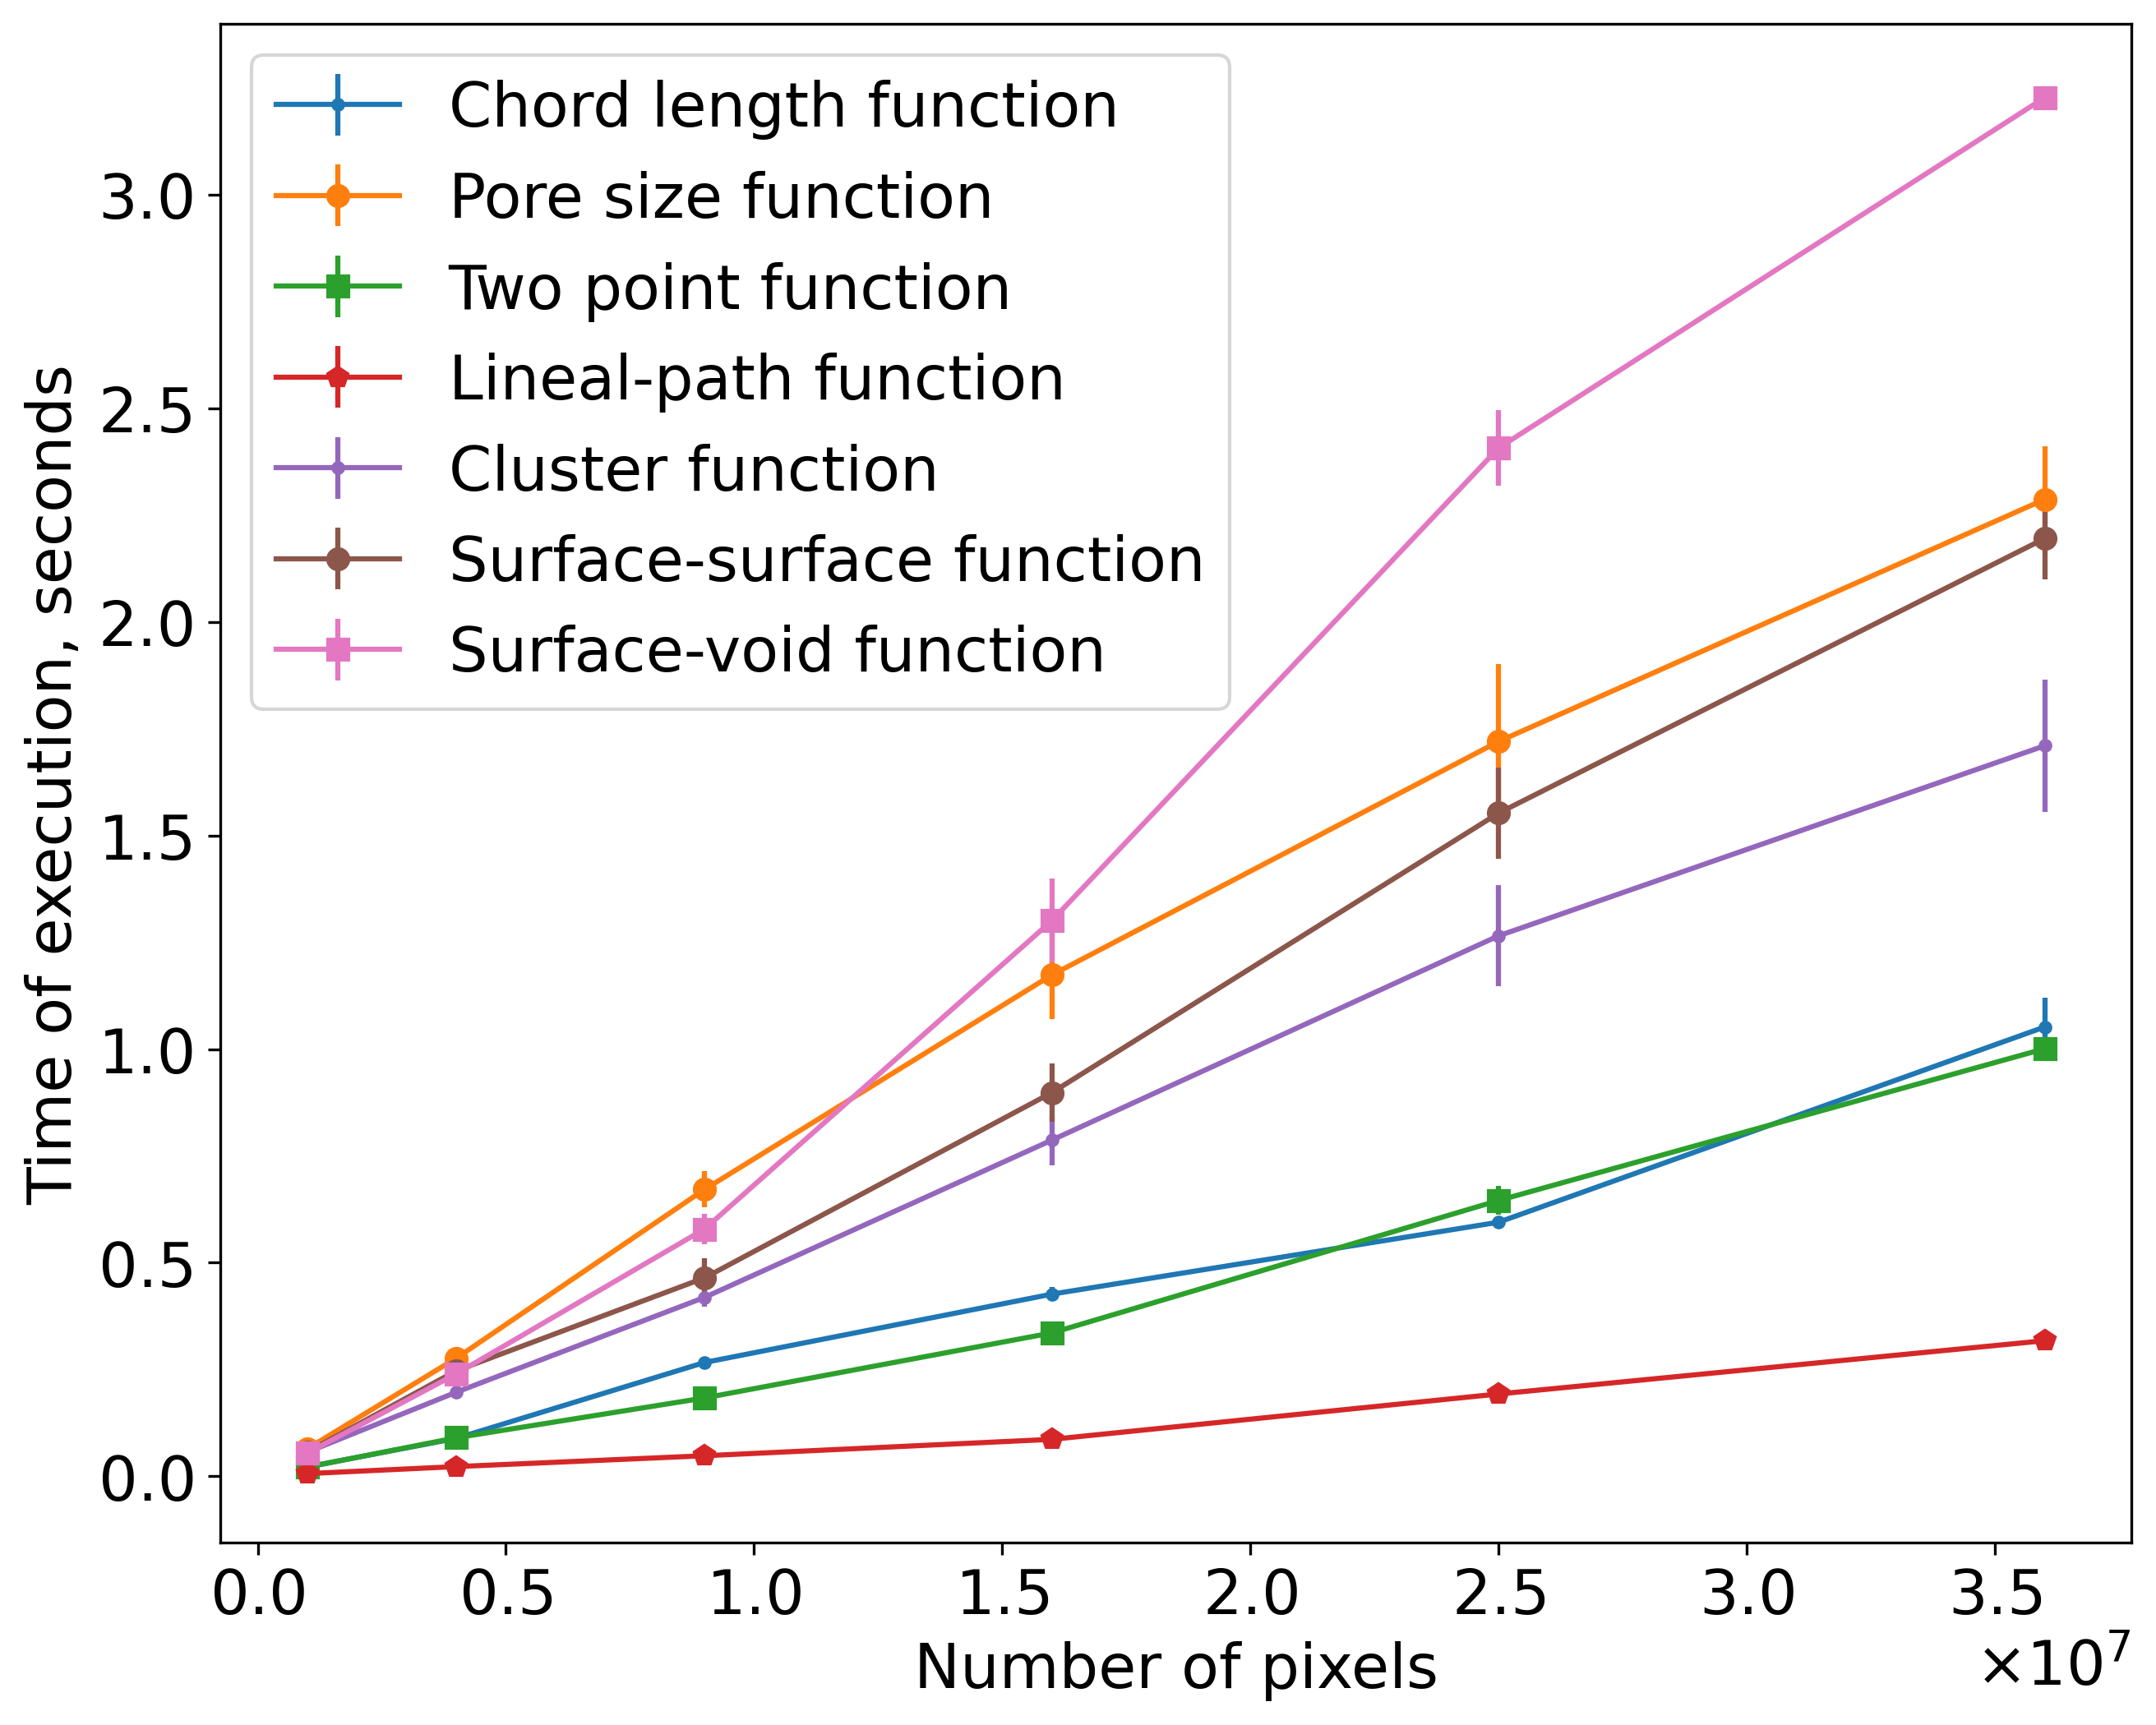
\includegraphics[width=\textwidth]{images/time-2d.png}
    \caption[]{{\small Two-dimensional case, module \code{Directional}}}
    \label{fig:timings-2d}
  \end{subfigure}
  \hfill
  \begin{subfigure}[b]{0.475\textwidth}
    \centering
    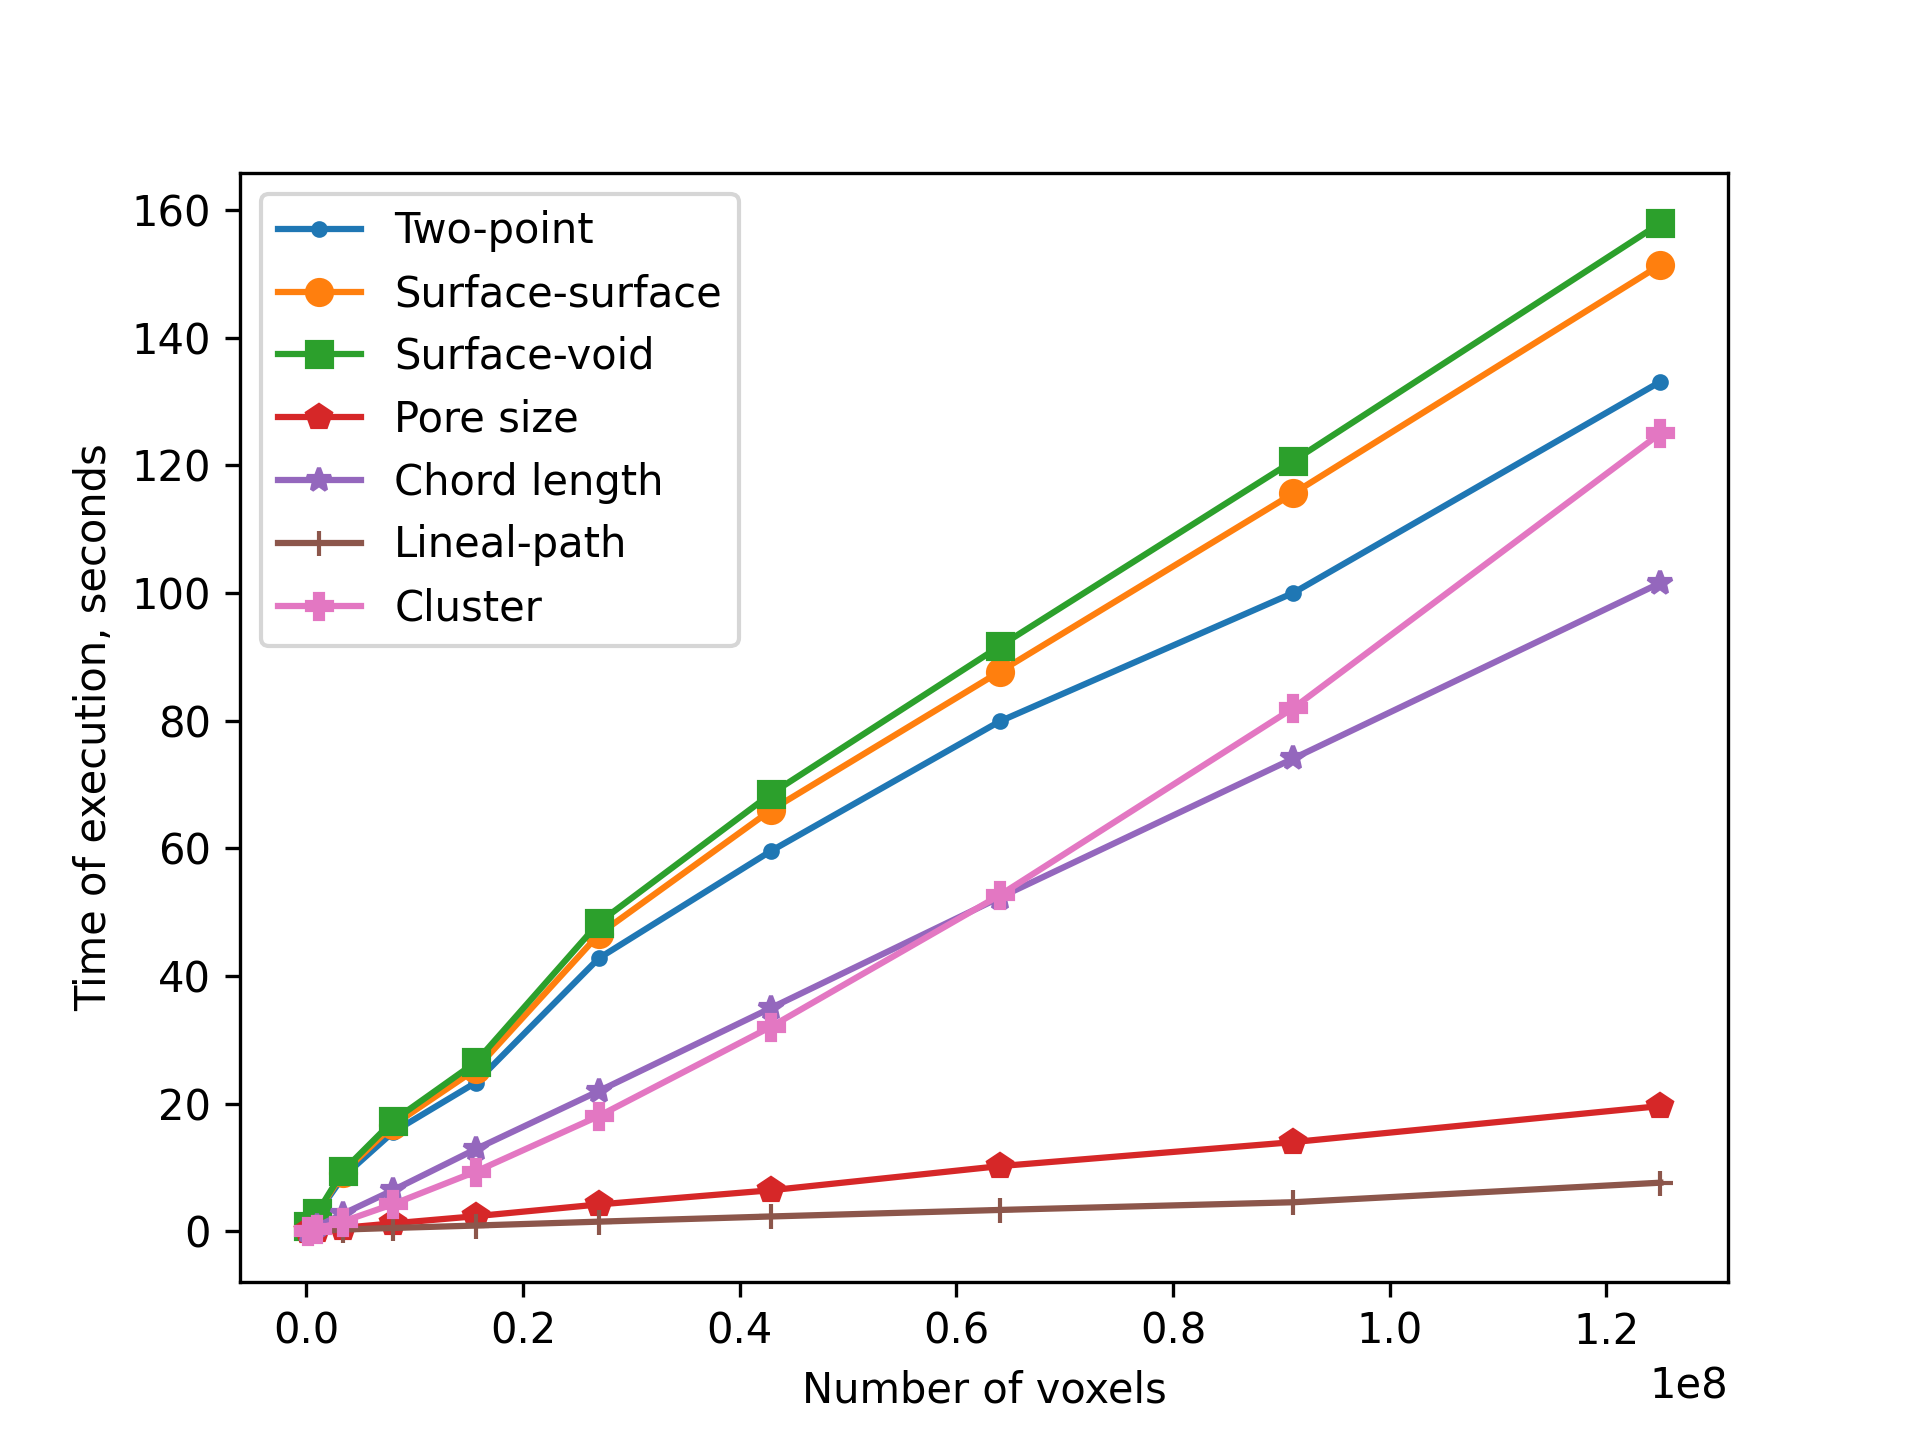
\includegraphics[width=\textwidth]{images/time-3d.png}
    \caption[]{{\small Three-dimensional case, module \code{Directional}}}
    \label{fig:timings-3d}
  \end{subfigure}
    \vskip\baselineskip
  \begin{subfigure}[b]{0.475\textwidth}
    \centering
    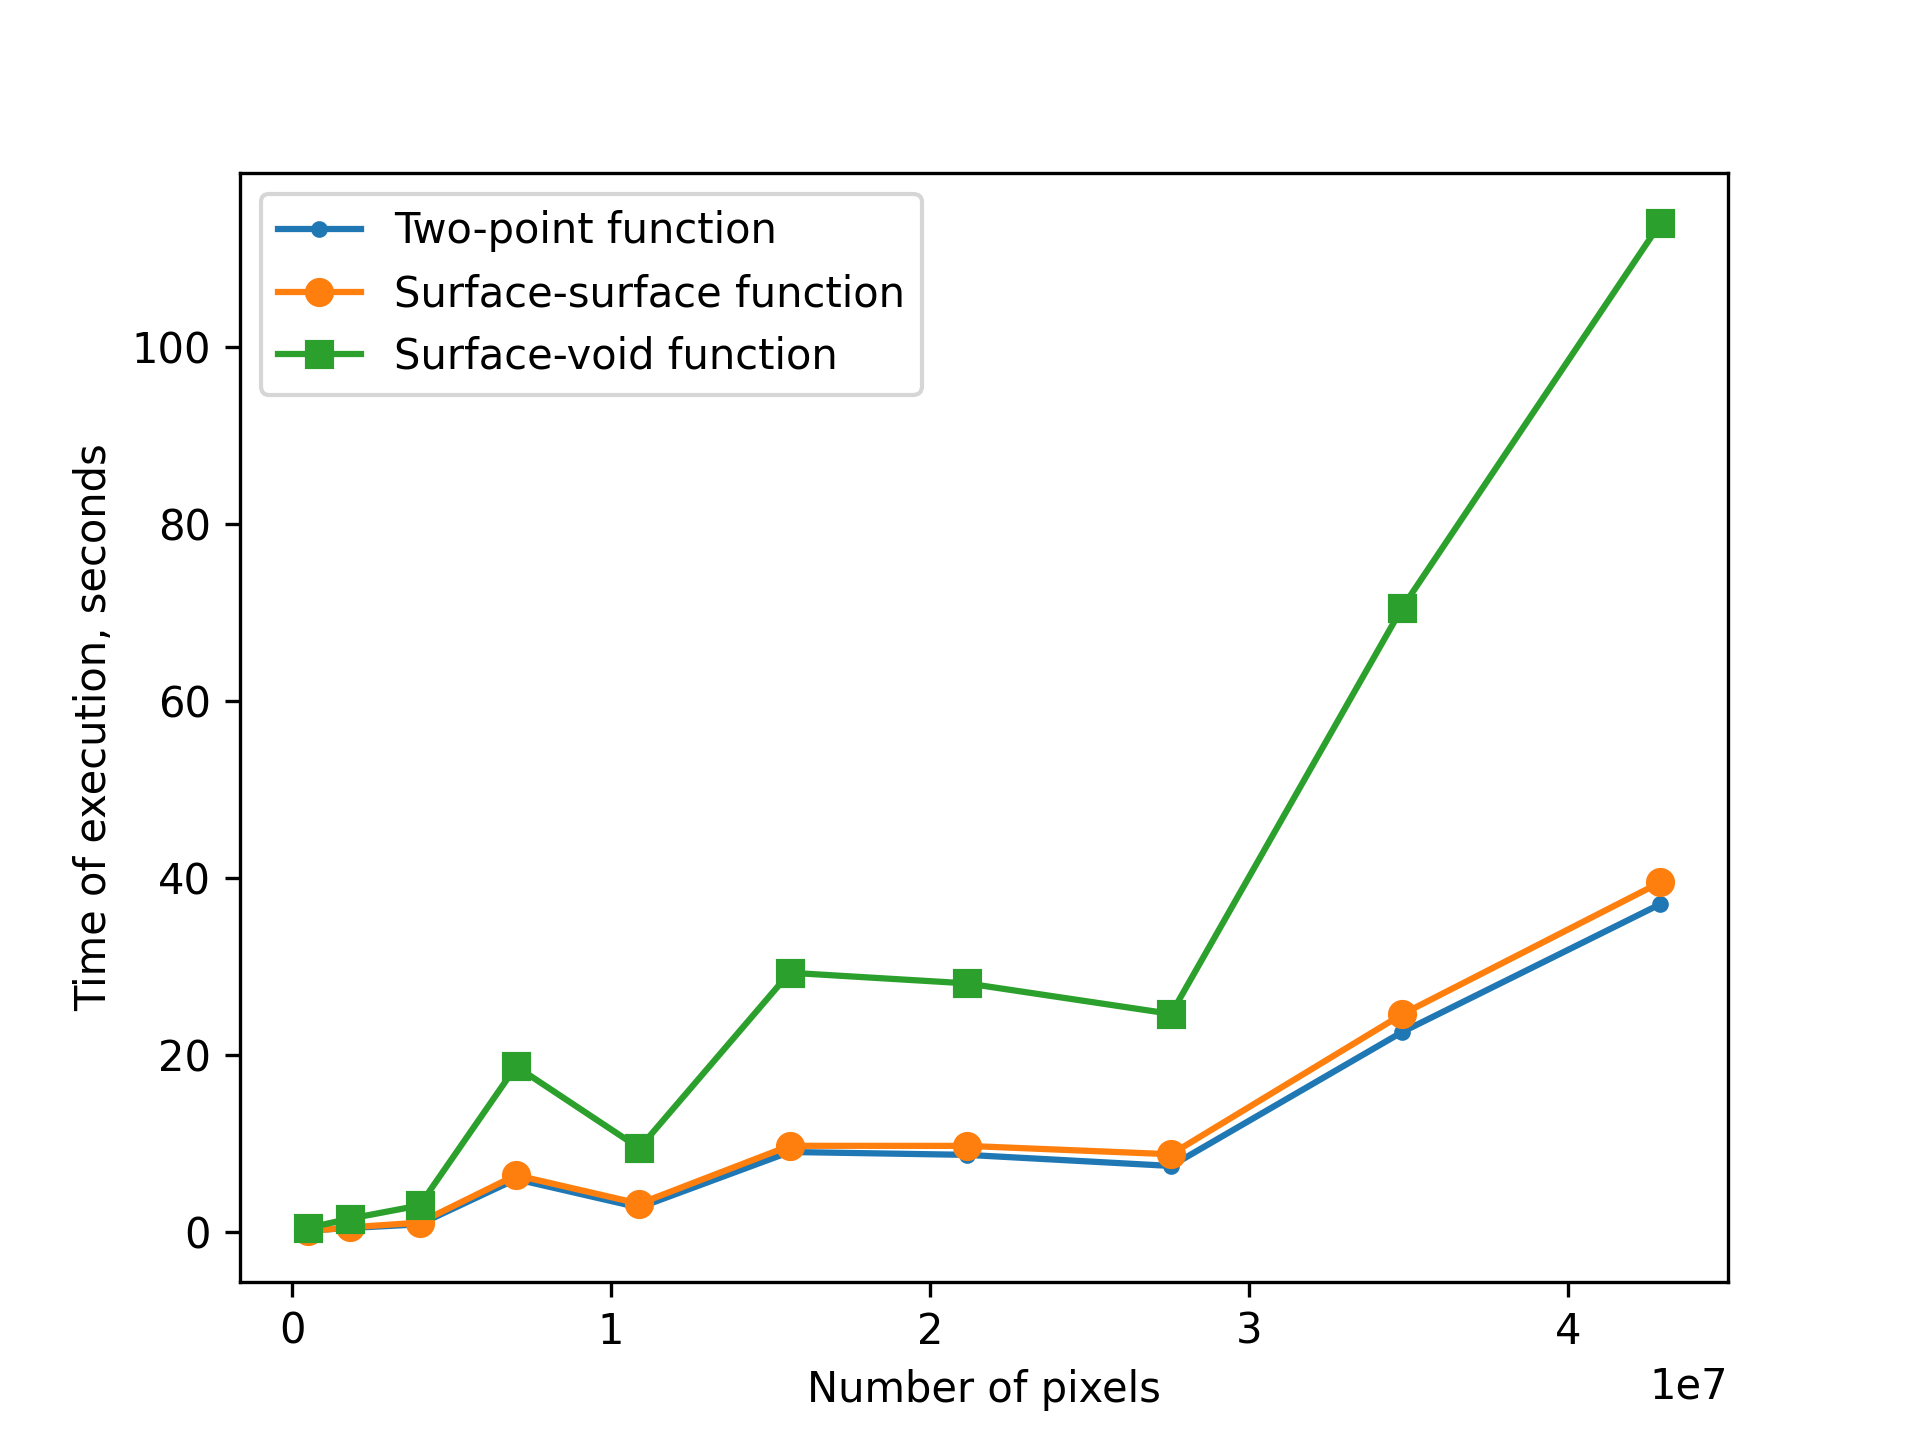
\includegraphics[width=\textwidth]{images/time-2d-map.png}
    \caption[]{{\small Two-dimensional case, module \code{Map}}}
    \label{fig:timings-2d-map}
  \end{subfigure}
  \hfill
  \begin{subfigure}[b]{0.475\textwidth}
    \centering
    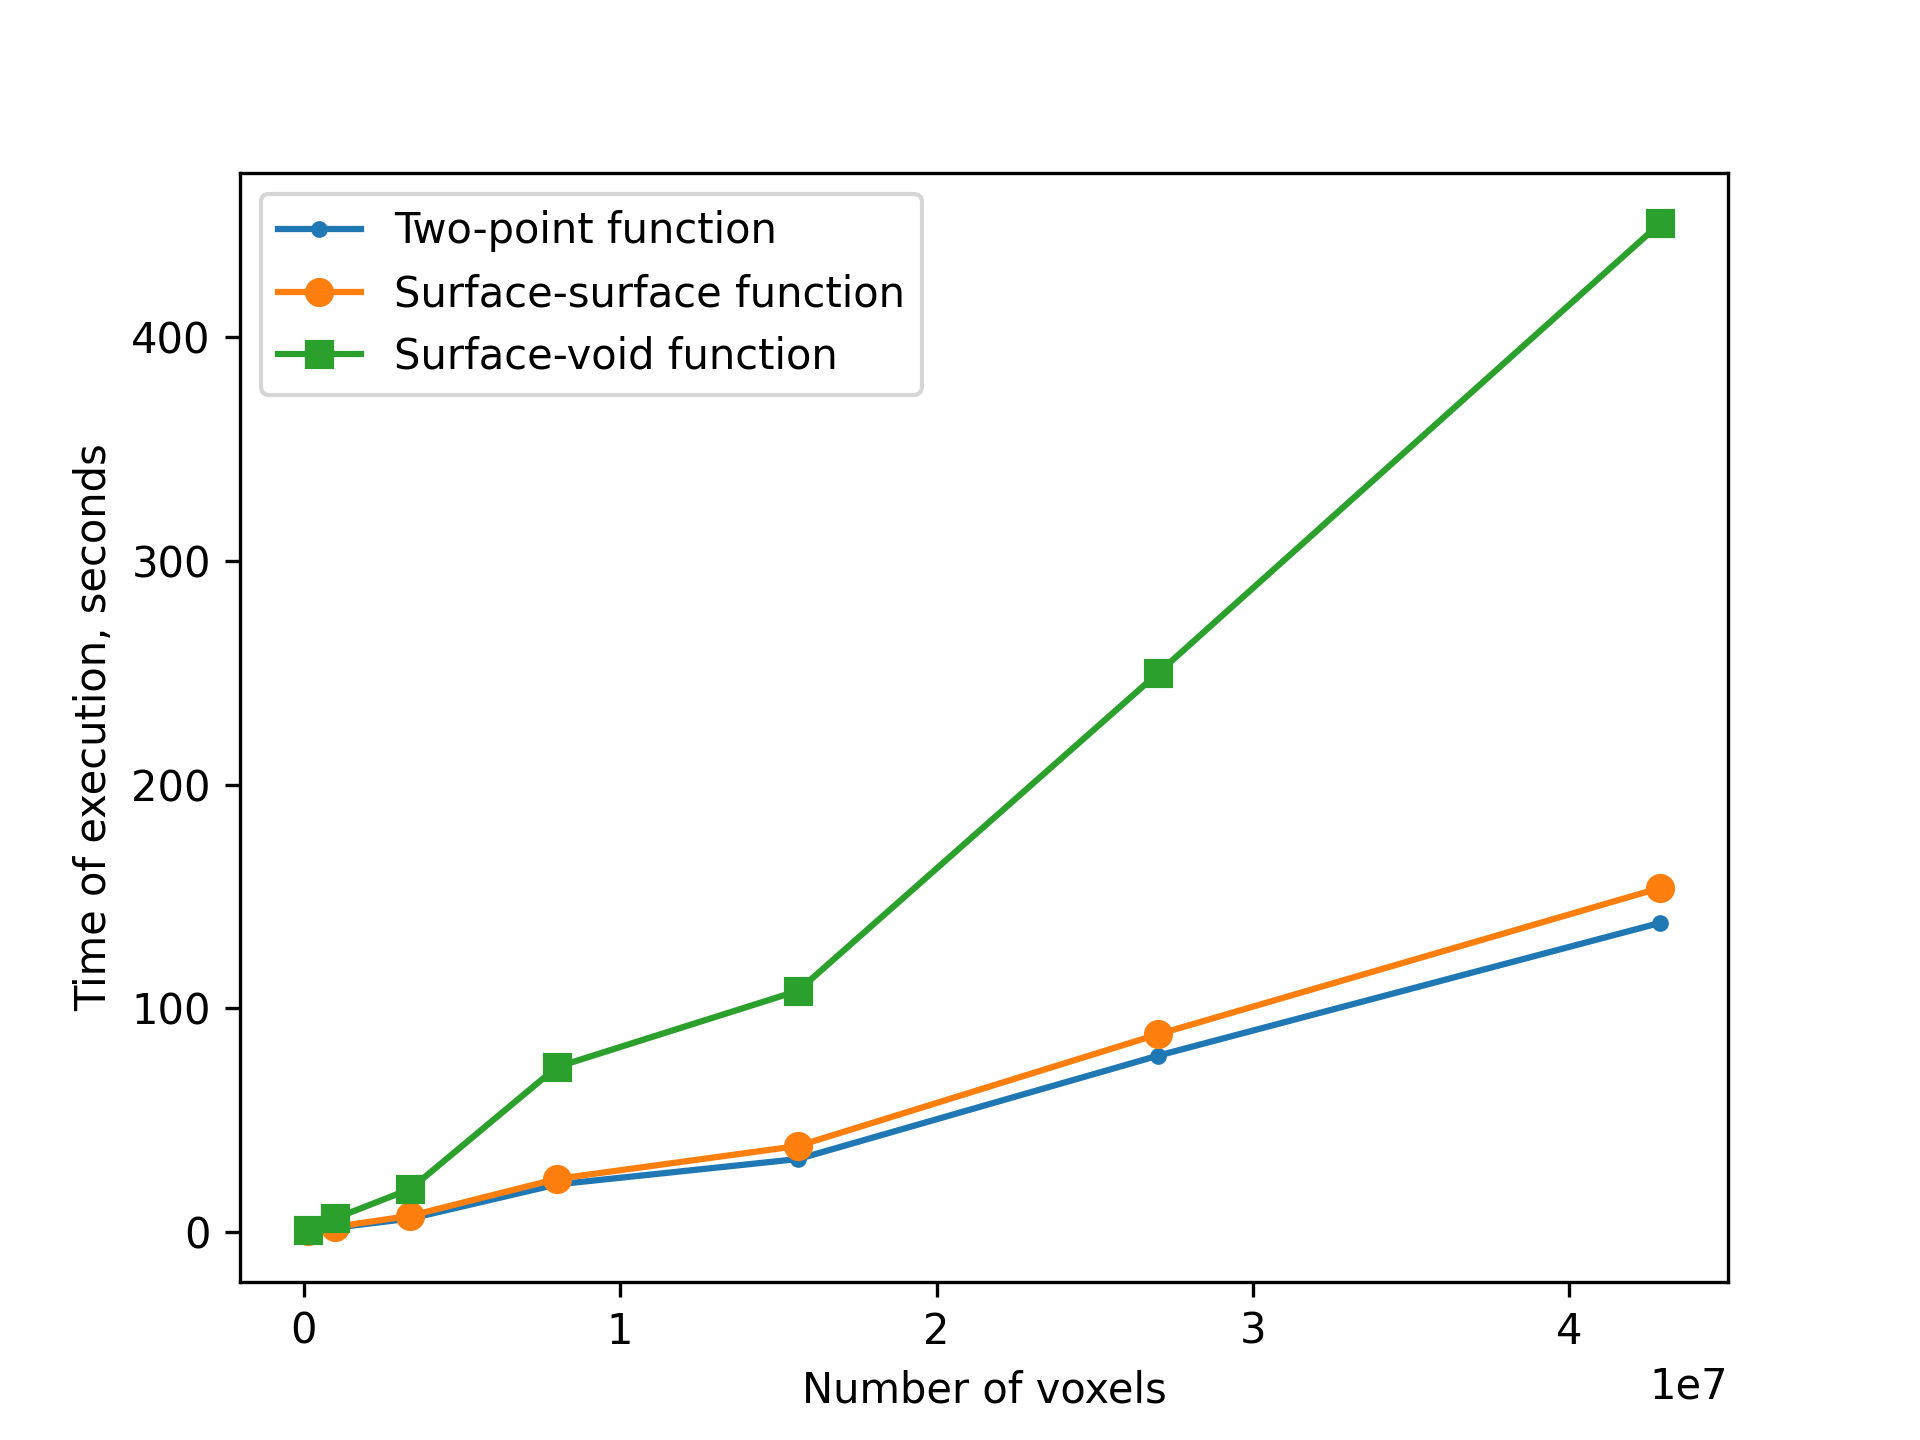
\includegraphics[width=\textwidth]{images/time-3d-map.png}
    \caption[]{{\small Three-dimensional case, module \code{Map}}}
    \label{fig:timings-3d-map}
  \end{subfigure}
  \caption[]{\small Execution times for different correlation functions.}
  \label{fig:timings}
\end{figure*}
\twocolumngrid

\appendix
\section{Algorithm of computation of lineal-phase function}
\label{linpathalg}
The algorithm below calculates $L_2^{(phase)}$ correlation function for
one-dimensional array $array$. The result is an array of $L_2$ values for
correlation lengths from $0$ to $maxlen-1$. If $periodic$ is true (resp. false)
then periodic (resp. CW) boundary conditions are used. The entry point of the
algorithm is the function L2. The efficiency of the proposed algorithm is $O(n)$
where $n$ is the length of the array.

\begin{algorithmic}[1]
  \Procedure{countruns}{$array, len, phase$}
    \State $runslist \gets [\quad]$
    \State $runs \gets 0$
    \ForAll{$x \in array$}
      \If{$x = phase$}
        \State $runs \gets runs + 1$
      \ElsIf{$runs \ne 0$}
        \State $runslist \gets runs:runslist$
        \State $runs \gets 0$
      \EndIf
    \EndFor
    \If{$runs \ne 0$}
      \State $runslist \gets runs:runslist$
    \EndIf
    \State \textbf{return} $runslist$
  \EndProcedure
  \\
  \Procedure{updateruns}{$array, runs, n$}
    \For{$idx = 1,n$}
      \State $array[idx] \gets array[idx] + runs$
      \State $runs \gets runs - 1$
    \EndFor
  \EndProcedure
  \\
  \Procedure{updateperiodic}{$array, first, last, n$}
    \State $sum \gets first + last$
    \State $n \gets \min(n, sum)$
    \For{$idx = 1,n$}
      \State $a \gets \min(idx - 1, first, last, sum - (idx - 1))$
      \State $array[idx] \gets array[idx] + a$
    \EndFor
  \EndProcedure
  \\
  \Procedure{l2}{$array, phase, maxlen, periodic$}
    \State $success \gets zeros(maxlen)$
    \State $total \gets zeros(maxlen)$
    \State $len \gets length(array)$
    \State $nupdates \gets \min(len, maxlen)$
    \State $runs \gets countruns(array, maxlen, phase)$
    \ForAll{$run \in runs$}
      \State $updateruns(success, run, \min(run, maxlen))$
    \EndFor
    \If{$periodic$}
      \State $first \gets first(array)$
      \State $last \gets last(array)$
      \If{$first = last$}
        \State $updateperiodic(success, first, last, nupdates)$
      \EndIf
      \State Increment $total[\text{from} \, 1 \, \text{to} \, nupdates]$ by
      $len$
    \Else
      \State $updateruns(total, len, nupdates)$
    \EndIf
    \State \textbf{return} $success$ divided by $total$ element-wise.  
  \EndProcedure
\end{algorithmic}
\end{document}
